\section{Architectural design}
\label{sect:overalldescription}

\subsection{Overview: High-level components and their interaction}
\label{subsect:Overview:Highlevelcomponentsandtheirinteraction}

The architecture of the system can be divided in three logical layers: \textbf{presentation layer}, \textbf{business layer} and \textbf{data layer}.

\begin{figure}[h!]
    \centering
    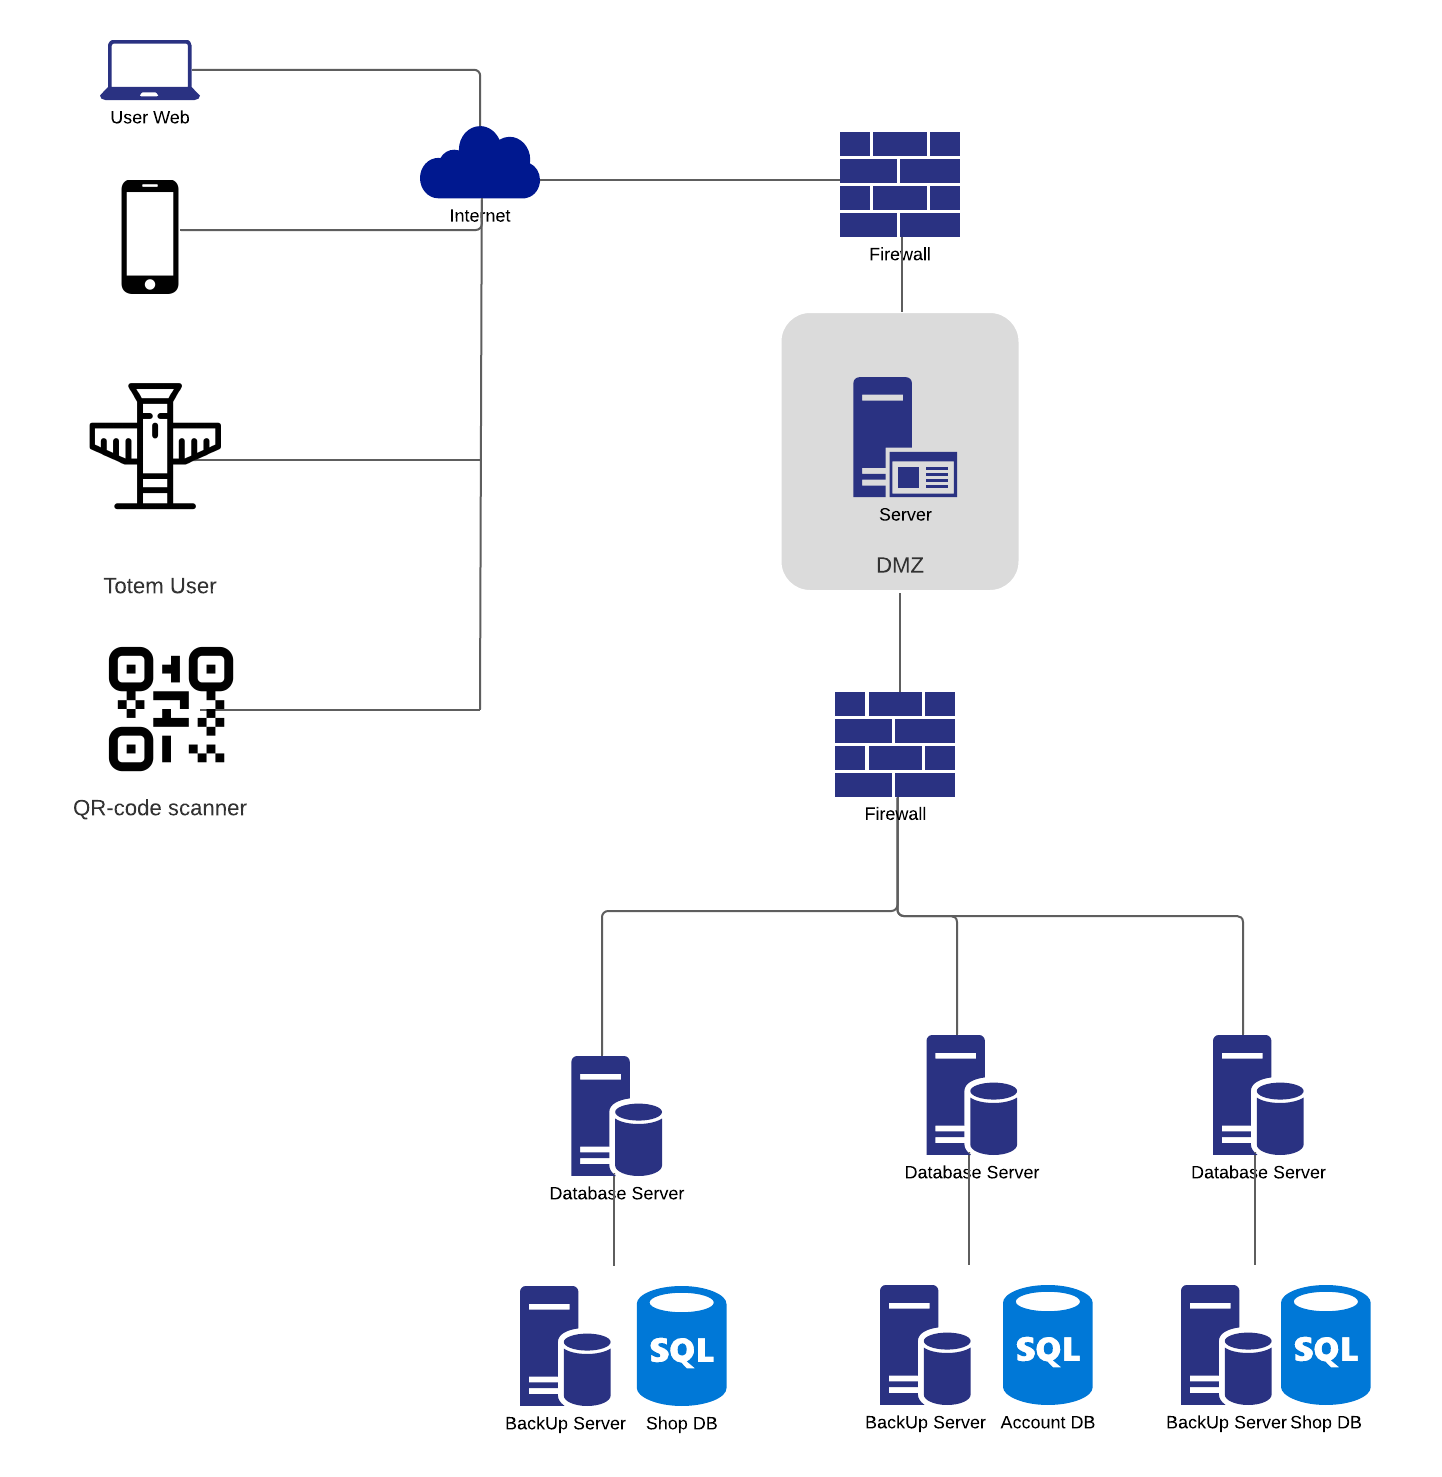
\includegraphics[width=0.75\textwidth]{Images/PhysicalDiagram.png}
    \caption{\label{fig:PhysicalDiagram}{Physical Diagram}}
\end{figure}

\FloatBarrier

The \textbf{presentation layer} is the part of the application that manages the interface through which the user will actually interact with our application. \newline
This layer will be managed either on client side, for what regards the offline functionalities and the static content display, and on server side, for what regards the dynamic content display. \newline
It has been chosen to develop a cross-platform application: in order to do so, the front-end of the application will be developed according with the framework of Redux in combination with React and React-Native.\newline
This means that the front-end will be supported either by IOs and Android Devices, as well as Web browsers.
Indeed, in the figure [\ref{fig:PhysicalDiagram}] we see that our users can connect with the server-side of the application via mobile devices, laptop devices, Totem devices and the Qr-code Scanner.\newline
Mobile devices will be able to connect either via their respective native application or the browser-based application.\newline
For what concerns the laptop users and the totem users, they will be able to connect to our application using only the browser-based application.\newline
Qr-code scanner application is a little more complicated and deserve a deeper explanation. It will be composed of two applications which will cooperate in order to correctly scan the Qr-code on the tickets and consequentially unlock the turnstills. One of the application, which will be implemented by us, will be just composed of a basic native UI and a QR-code scanner, while the underlaying application will provide the unlock and lock of the turnstills.\newline
The latter won't be discussed in this document any further since it's not under our supervision.

The \textbf{Business layer} is the core of the application and connect the presentation layer and the data layer. It allows users to retrieve desired data and to have access to dedicated functionalities. We decided to implement our business layer using the Micro-Services architecture. This architecture divides the application in multiple tinier applications, each of which is mainly dedicated to a specific function. All of those micro-services coadiuvate in order to offer to the user the entire set of features offered by the application. This is the best way to implement an application which must be scalable, as CLup, which is a young start-up hoping to grow a lot. Furthermore, we decided to implement a cloud computing based application: through the joined use of Kubernetes and Docker it is possible to scale the resources needed dynamically and according to the incoming requests, so that, with a IaaS approach, we will be able to reduce the costs to the essential.

By the way, each of our micro-services will need, in order to fulfill its duty, to store and retrieve several information. This information will be kept in dedicated SQL Data Bases, which represents, jointed with the SQL DBMS, the \textbf{Data Layer}. The data layer is the memory of our application and a significant part of it, for this reason for each database a Backup database will be implemented either.

\subsection{Component view}
\label{subsect:componentview}

The following diagrams [\ref{fig:ComponentViewHighLevel}] show the main components of the system and the interfaces through which they interact. The coloured ones are the one we are going to implement:

\begin{itemize}[topsep=0pt]
    \item The client side is made of four components, which refer to the qr-code scanner application, to the web users and to the mobile application users.
    \item The server side is divided in three subsystems, each of them implements a specific service of the application. For the sake of clarity three different diagram has been modelled. The subsystems are:
    \begin{itemize}[topsep=0pt]
        \item the \textbf{Queue Services Subsystem}: provides the interfaces needed either by managers and users in order to accesses to the functions correlated to the queue associated to a shop. 
        \item the \textbf{Shop Services Subsystem}: provides the interfaces needed by managers and users in order to access the functions correlated to a shop.
        \item the \textbf{Account Manager Services}: provides the interfaces needed to manage the accounts and also implements some security features.
    \end{itemize}
\end{itemize}

\begin{figure}[h!]
    \centering
    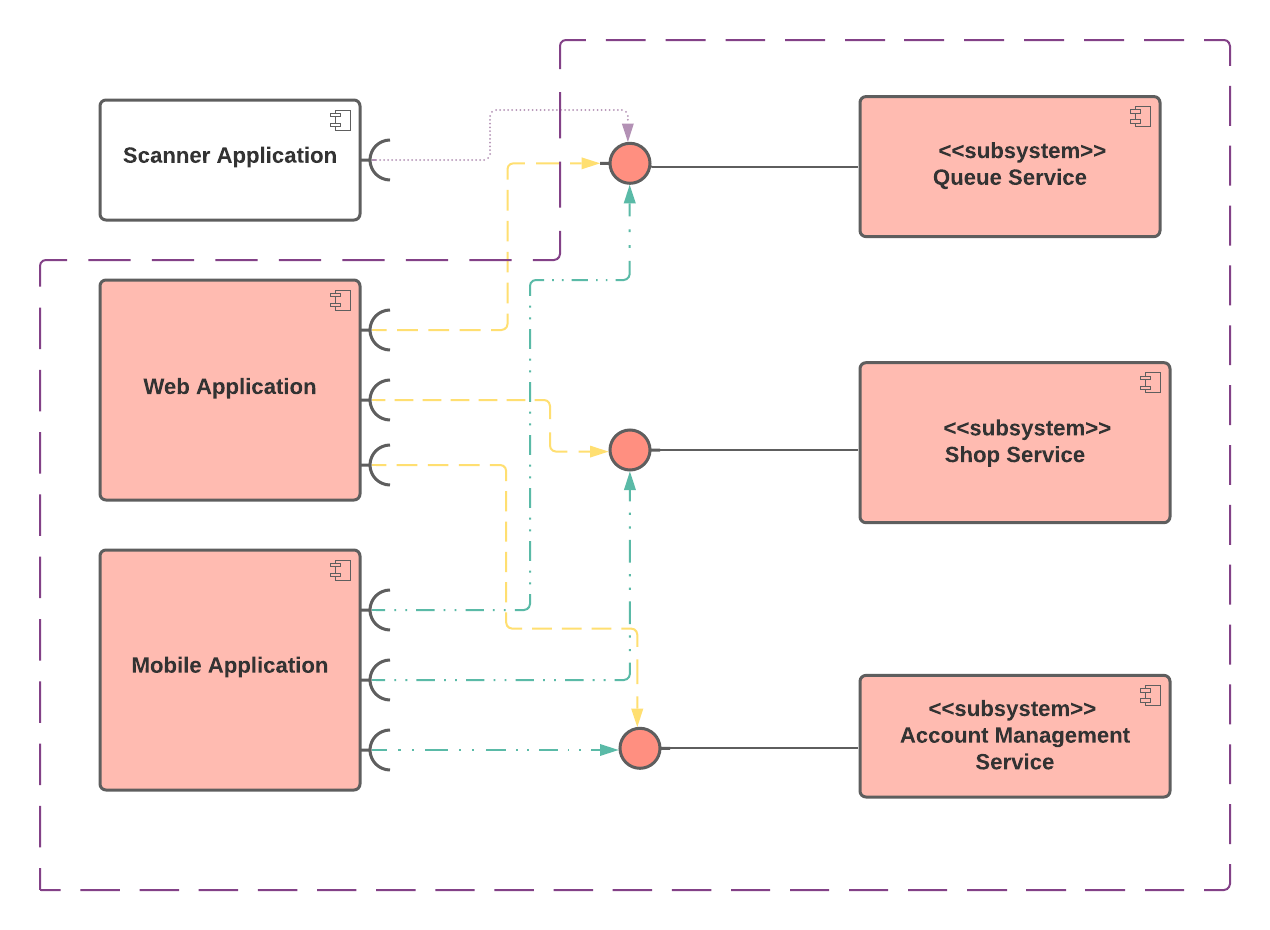
\includegraphics[width=0.7\textwidth]{Images/ComponentViewHighLevel(1).png}
    \caption{\label{fig:ComponentViewHighLevel}{General component view}}
\end{figure}

\FloatBarrier

\subsubsection{Queue Service Subsystem Projection}
\label{subsubsect:queueservice}

This service is divided in several components: \textit{Qr-code scanner component, Visit component, LineUp Component, Queue Info Component, Analytics Component, Ticket Generator Component, Notificate User Component and Data Manager Component}. 

\begin{figure}[h!]
    \centering
    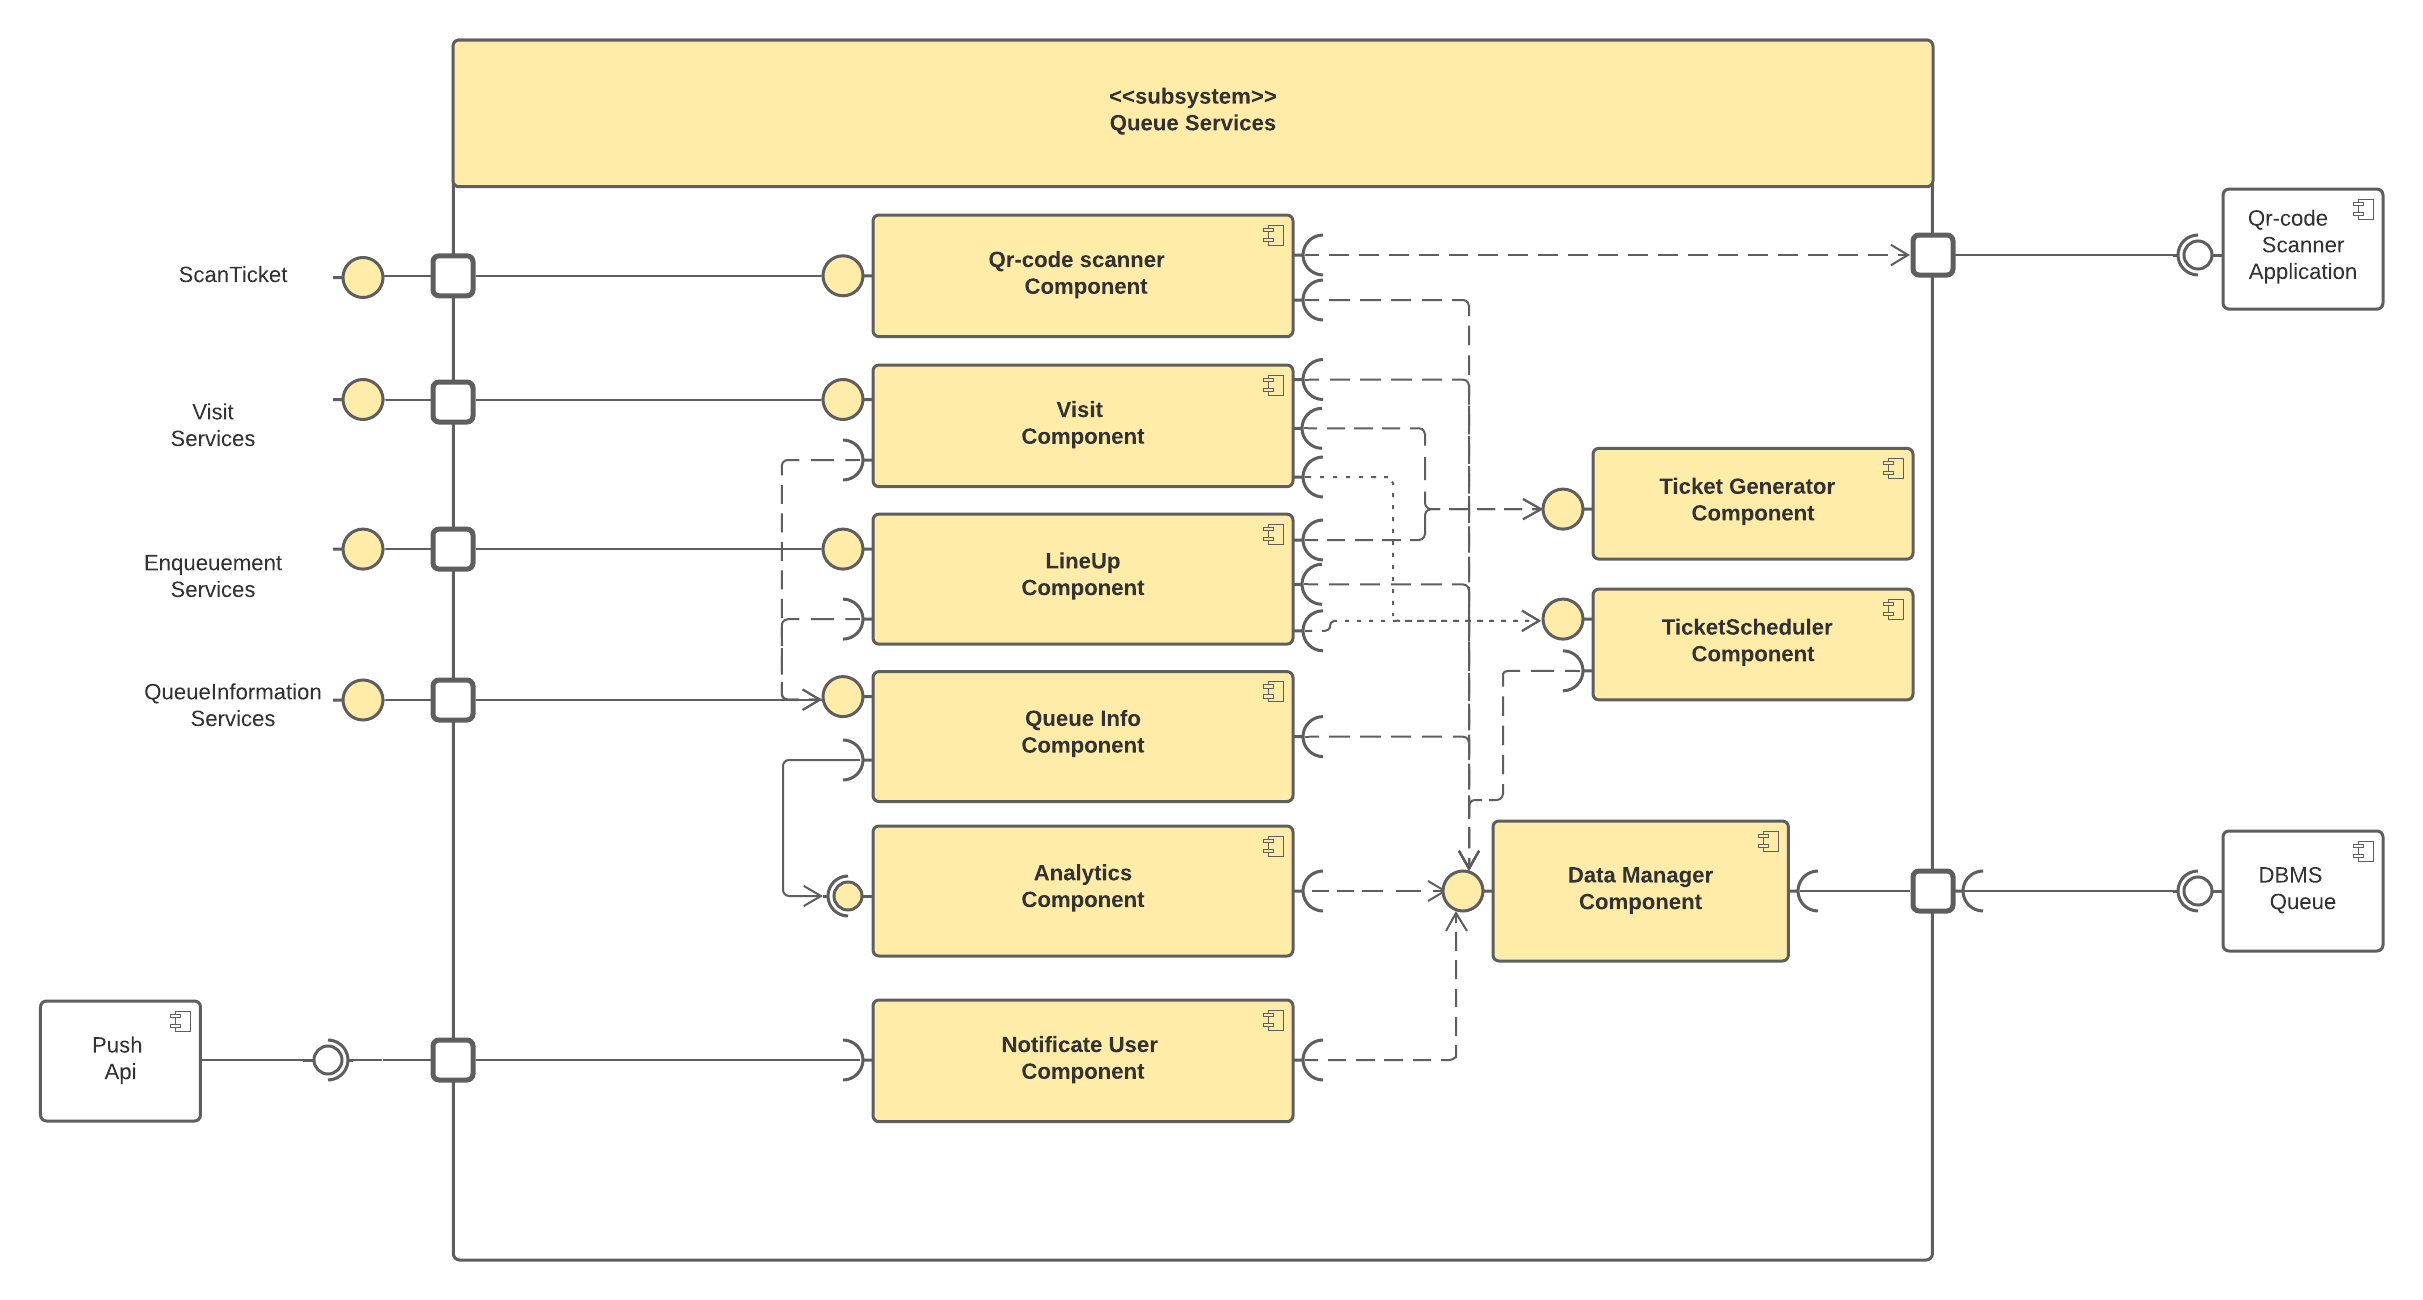
\includegraphics[width=0.9\textwidth]{Images/ComponentViewQueueService(1).png}
    \caption{\label{fig:ComponentViewQueueServices}{Queue Service Component}}
\end{figure}

\FloatBarrier

The \textbf{Qr-code scanner Component} is a component dedicated to update the status of the ticket once they are scanned. It communicates with the QR-code scanner, offering it an interface through which it will be able to call it, in order to correctly fulfill its function.

The \textbf{Visit Component} is a component dedicated to the management of the visit tickets. It generate a ticket through the \textit{Ticket Generator Component} and decorate it as a visit ticket. It offers to the client a set of functionalities, such as book a visit or cancel a previous booked one.

The \textbf{LineUp Component} is a component dedicated to the management of the queue tickets. It generates a ticket through the \textit{Ticket Generator Component} and decorate it as a queue ticket. It offers to the client a set of functionalities, such as the possibility to enqueue or to dequeue in the virtual queue.

The \textbf{TicketScheduler Component} is a component dedicated to the update of the queue. If offers an interface to the \textit{LineUp Component} and to the \textit{Visit Component} and interact with the \textit{DataManager Component}. Indeed, it offers a dedicated interface to the clients.

The \textbf{Queue Info Component} is a component dedicated to the retrievement of the information about the queue of a shop.
Indeed, it offers a dedicated interface to the clients. It may have the need to handle immediate information or analytical data. The latter, are calculated thanks to the \textit{Analytics Component}.

The \textbf{Analytics Component} is a component dedicated to the computation of analytical data about the queue.

The \textbf{Notificate User Component} is a component dedicated to the task of sending push notifications to clients. In order to so, it communicates with a Push Api.

Finally, the \textbf{Data Manager Component} is a component dedicated to interact with the Queue DBMS and offers an interface to all of the other component in the service in order to have access to it.

\subsubsection{Shop Service Subsystem Projection}
\label{susbsubsect:shopservice}

This service is divided in three components: \textbf{Manage Shop Component, Shop Info Module, Data Manager Module}.

\begin{figure}[h!]
    \centering
    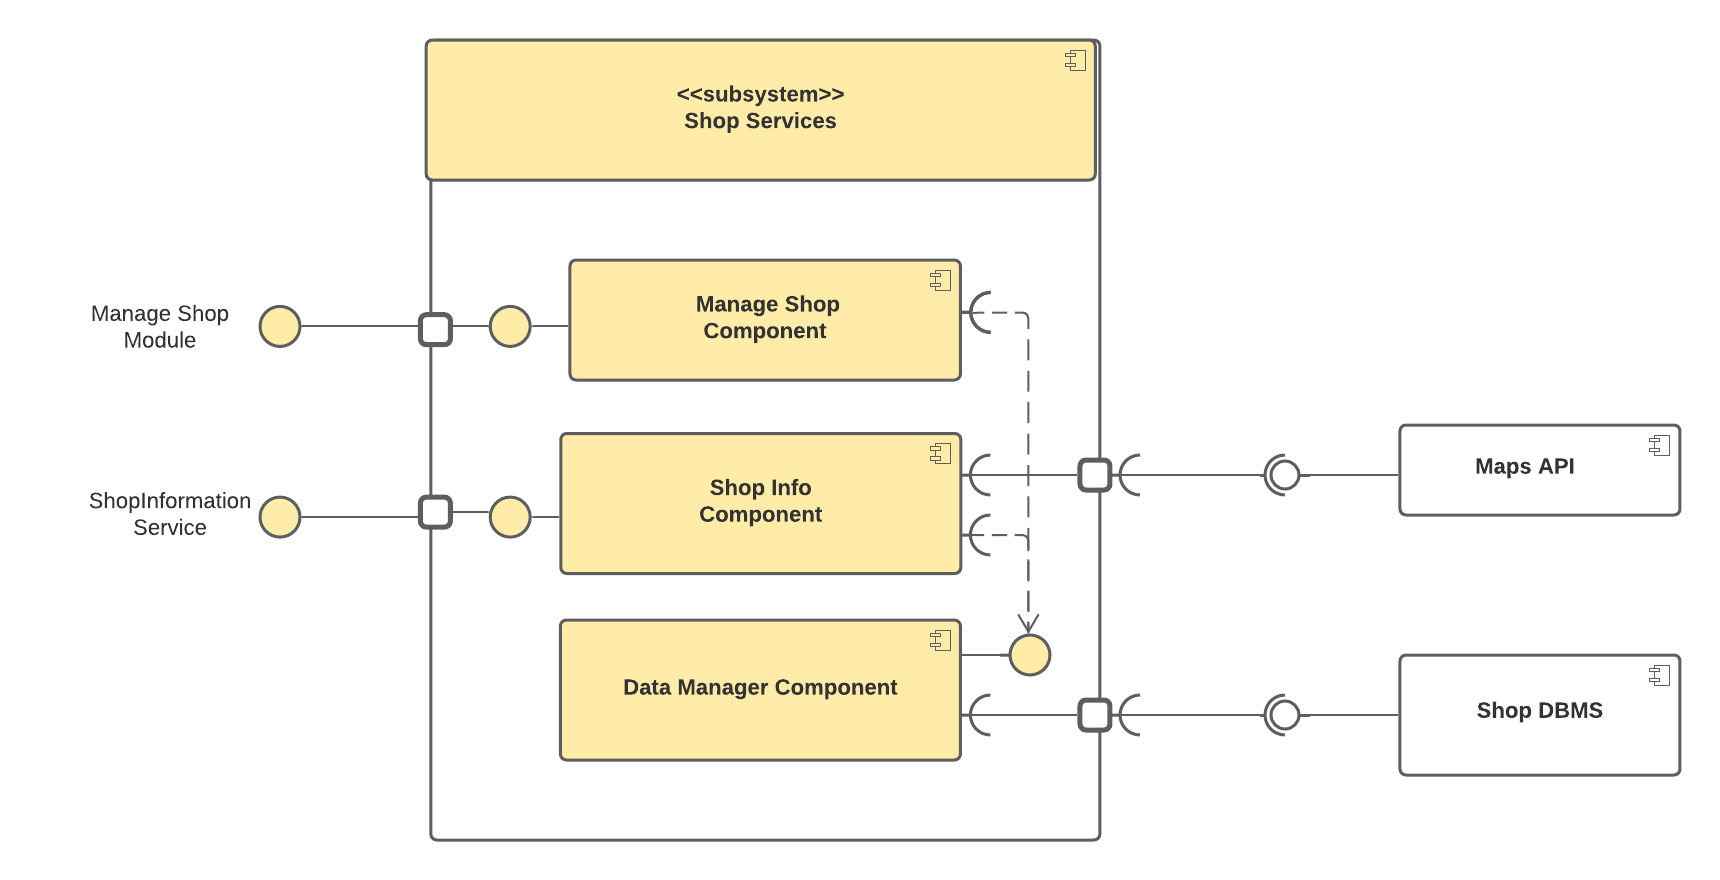
\includegraphics[width=0.9\textwidth]{Images/ComponentViewShopServices(1).png}
    \caption{\label{fig:ComponentViewShopServices}{Shop Services Component}}
\end{figure}

\FloatBarrier

The \textbf{Manage Shop Component} is a component dedicated to implement features exploited mainly by the managers. It implements an interface which will allow a manager to add a shop and to update the information of a shop already registered in the system.

The \textbf{Shop Info Component} is a component which implements an interface that provides functions to retrieve information about a shop. This component, for some of its features, needs to communicate with the Maps Api.

Finally, the \textbf{Data Manager Component} is a component dedicated to interact with the Shop DBMS and offers an interface to all the other component in the service in order to have access to it.

\subsubsection{Account Manager Subsystem Projection}
\label{subsubsect:accountmanagerservice}

This service is divided in three components: \textbf{Account Manager Component, Authentication and Authorization Engine Component and the Data Manager Component}.

\begin{figure}[h!]
    \centering
    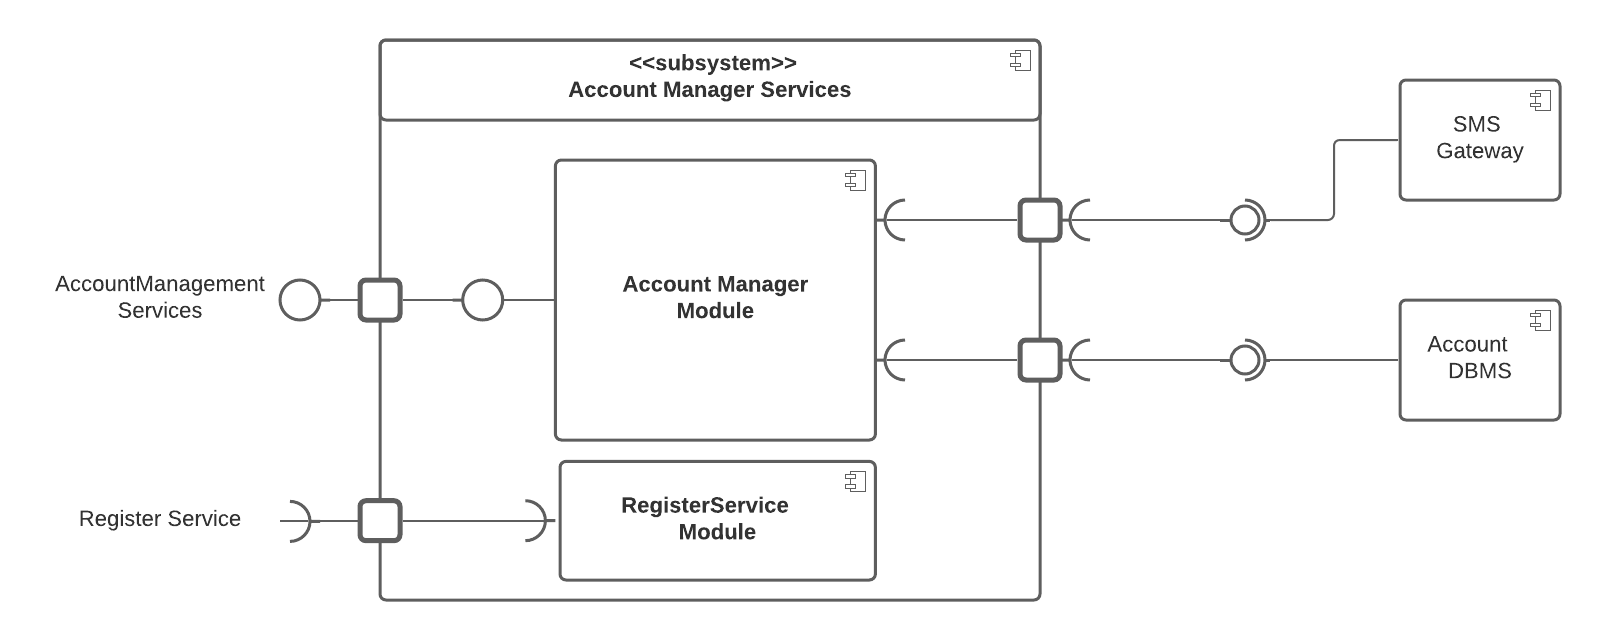
\includegraphics[width=0.9\textwidth]{Images/AccountManagerServices.png}
    \caption{\label{fig:ComponentViewAccountManagerServices}{Account Manager Services Component}}
\end{figure}

\FloatBarrier

The \textbf{Account Manager Component} is a component dedicated to manage the users' accounts. It offers the users an interface through which they can, for example, sign on, sign in or update their profile. 

It communicates with the \textbf{Authentication and Authorization Engine Component} which provides an interface with the functions needed in order to identify and authenticate a user. It will need to communicate with the SMS gateway from time to time in order to accomplish its functions.

The \textbf{Data Manager Component} is a component dedicated to interact with the Account DBMS and offers an interface to all of the other component in the service in order to have access to it. 

\subsection{Entity-relationship diagram}
\label{subsect:entityrelationshipdiagram}

\subsection{Deployment view}
\label{subsect:deploymentview}

The system architecture is a 3-Tier architecture, it is based on the JEE framework and it's typical of a Service Oriented Application:

\begin{itemize}[topsep=0pt]
    \item \textbf{TIER 1} is the client tier, it is composed of the mobile applications, the totems and the users browsers and the qr-code scanner application. All of them will communicate with the web server via the HTTPS protocol.
    \item \textbf{TIER 2} is composed of the application server. This tier hosts the OS system CentOs, which will welcome the platform Kubernetes which, with the joint effort of Docker, will orchestrate the ideal enviroment execution for our microservices application. Kubernetes, among its numerous services, offers an ELB api, through which will successfully dispatch correctly the incoming HTTP requests to the correct service. Each service will be deployed as a Docker Image directly by Kubernetes through a Docker File and will be hosted in a Docker container.
    \item \textbf{TIER 3} is the Data Tier. 
    We decided to implement 3 different Databases, one for each offered microservice. 
    The connection beetween Tier 2 and 3 is performed via JDBC connector which uses jdbc protocol.
\end{itemize}

\begin{figure}[h!]
    \centering
    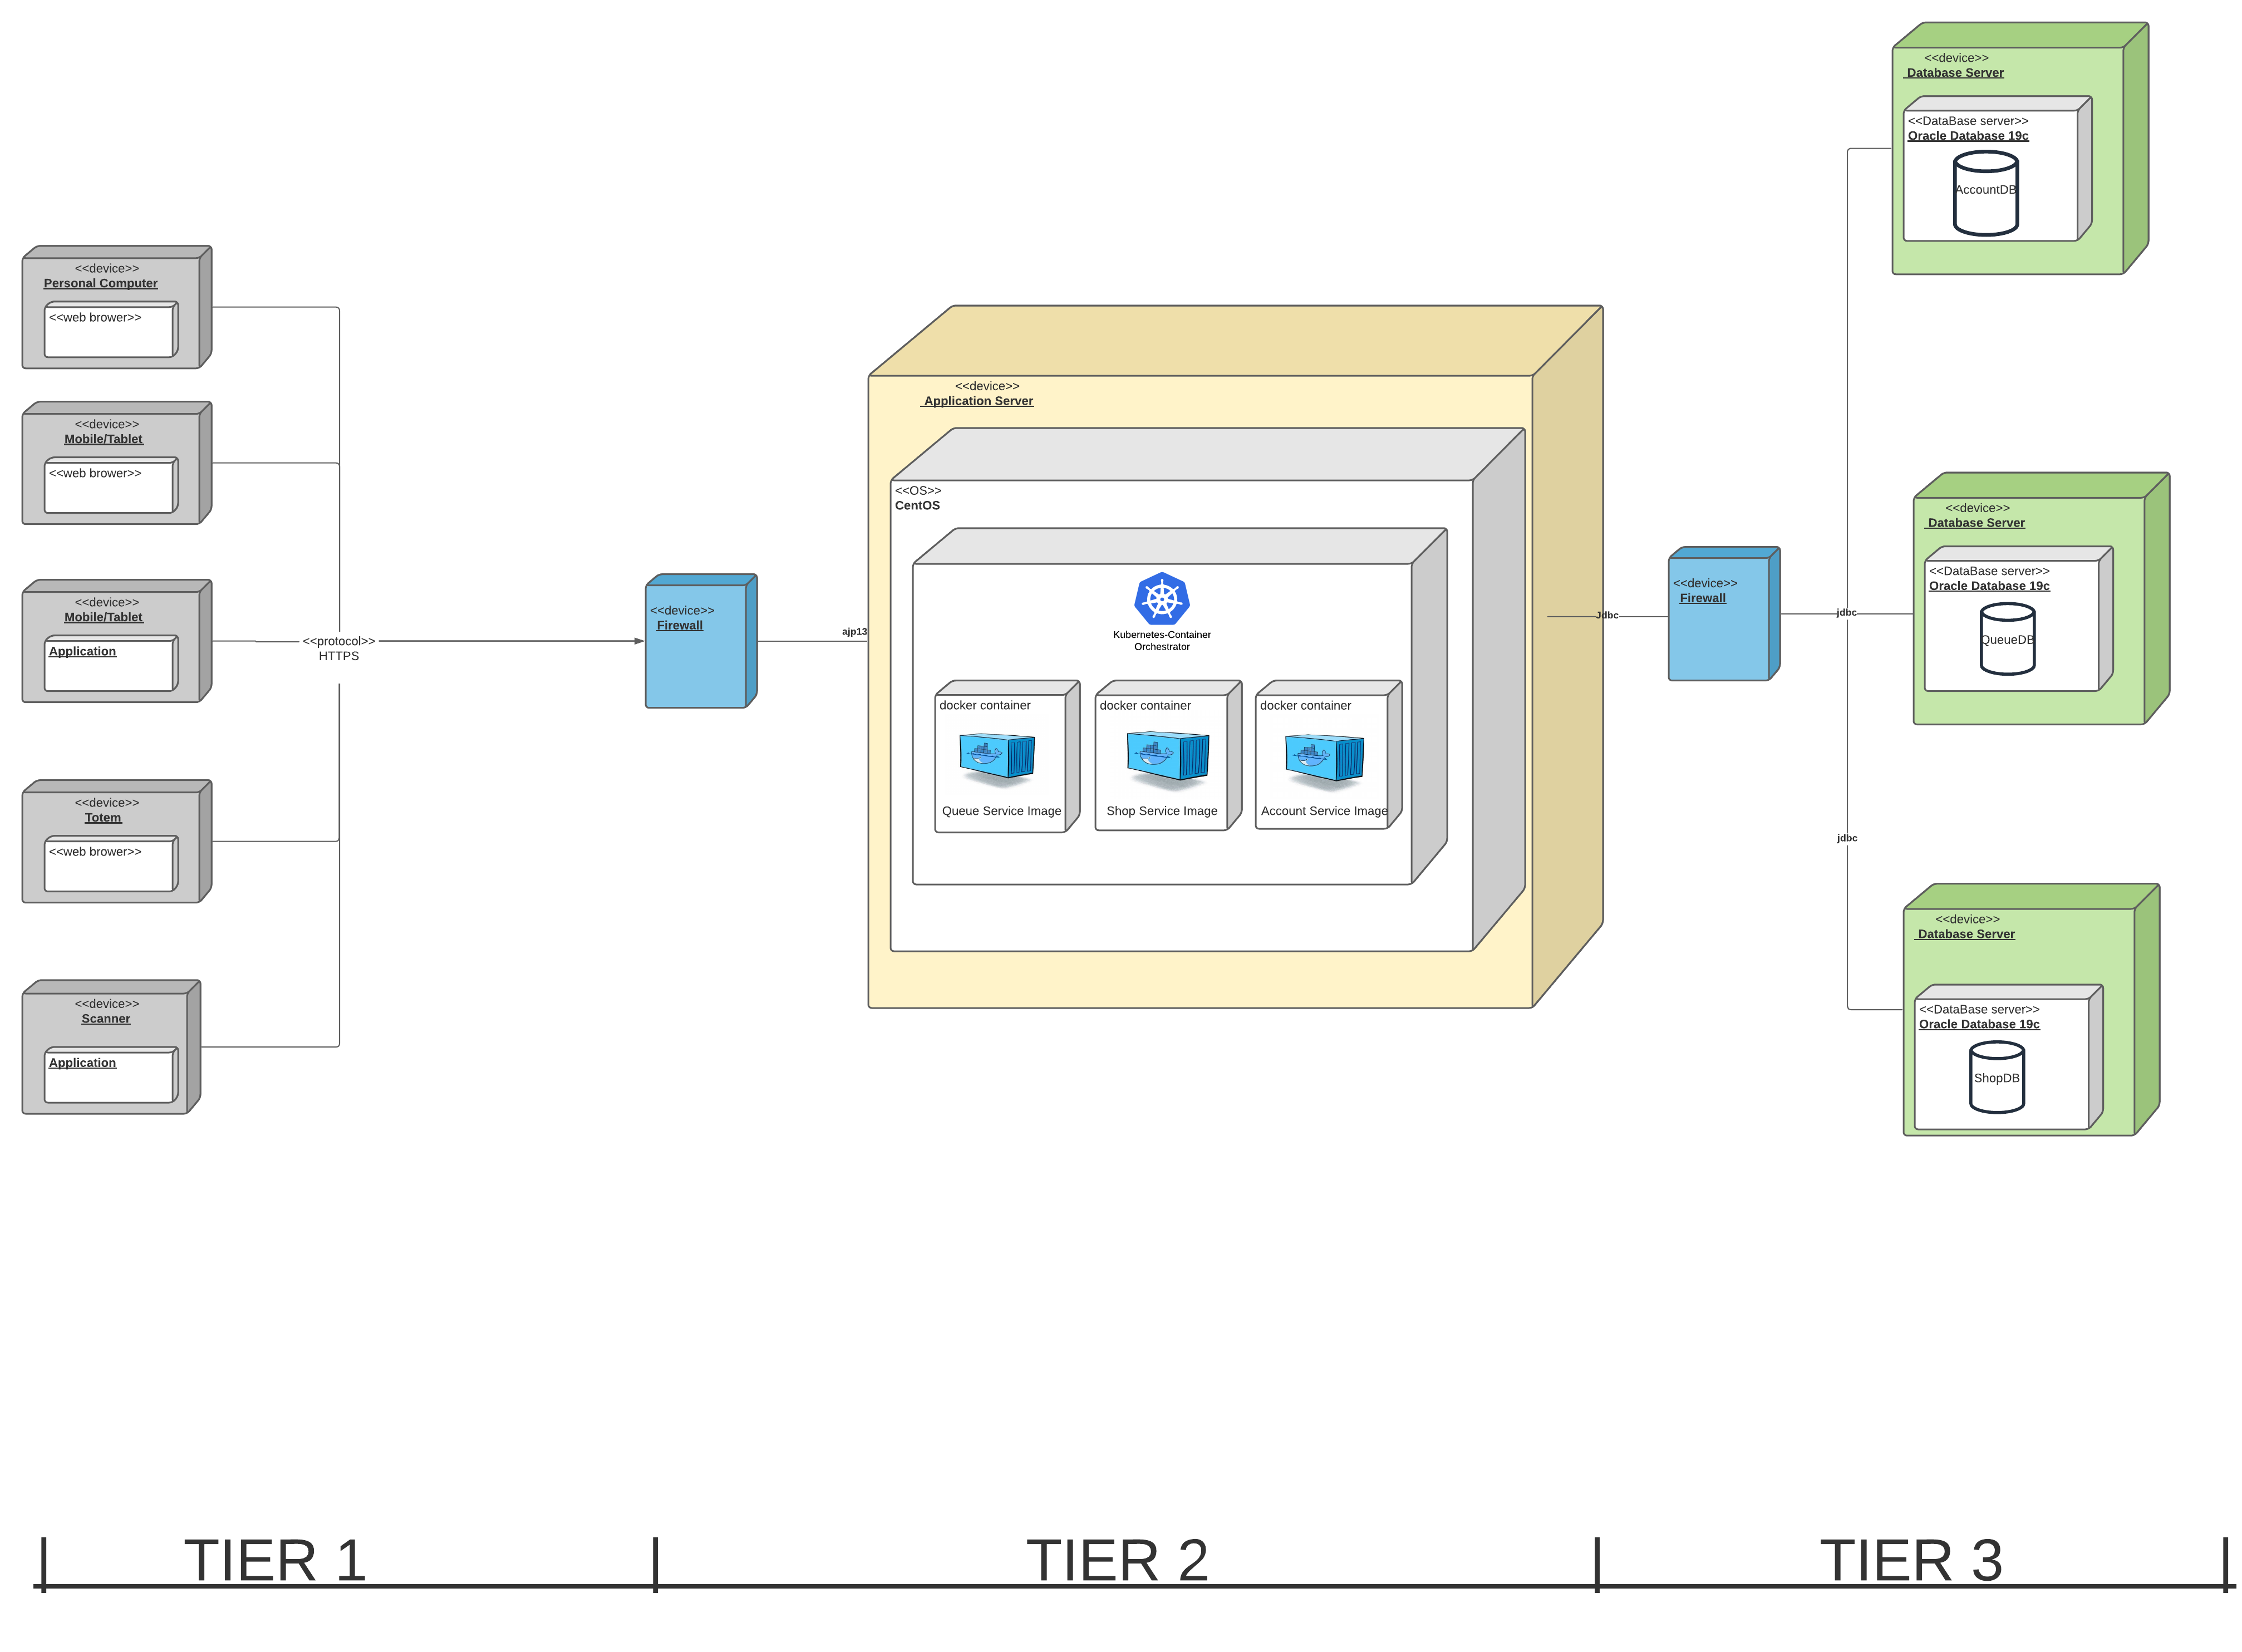
\includegraphics[width=0.9\textwidth]{Images/Deployementview(2).png}
    \caption{\label{fig:Deployement View}{3-Tier Architecture}}
\end{figure}

\FloatBarrier

\subsection{Runtime view}
\label{subsect:runtimeview}

The following sequence diagrams describe the interaction between the main components of the system in some of the most common use case scenarios. It is very important to highlight that these diagrams have no intention of specifying the detailed behavior of our product, but they have just an illustrative purpose. Indeed, their aim is to clarify with approximate sketches some of the interactions that may occur between the user and the system and, inside the latter, between the components.
For this reason, some of the trivial thus fundamental behavior of the system have been omitted. 

Between these, we want to specify in these instance the main two significant ones that the reader may find strange not to find in the diagrams.

First of all, we reassure the reader that all the data inserted in the forms compiled at client side will be verified also at server side, even if these checks aren't always represented.\newline
In second instance all the features that will affect the queue of a shop- some of them in sequence diagrams 2,3,4- TicketScheduler Component in Queue Service Subsytem will be called and will perform the dedicated algorithm in order to update the queue. This will also trigger the push notifications to all the users involved through the Push Api.

With these premises, we shall let the reader continue their inspection of the following diagrams.

\begin{figure}[h!]
    \centering
    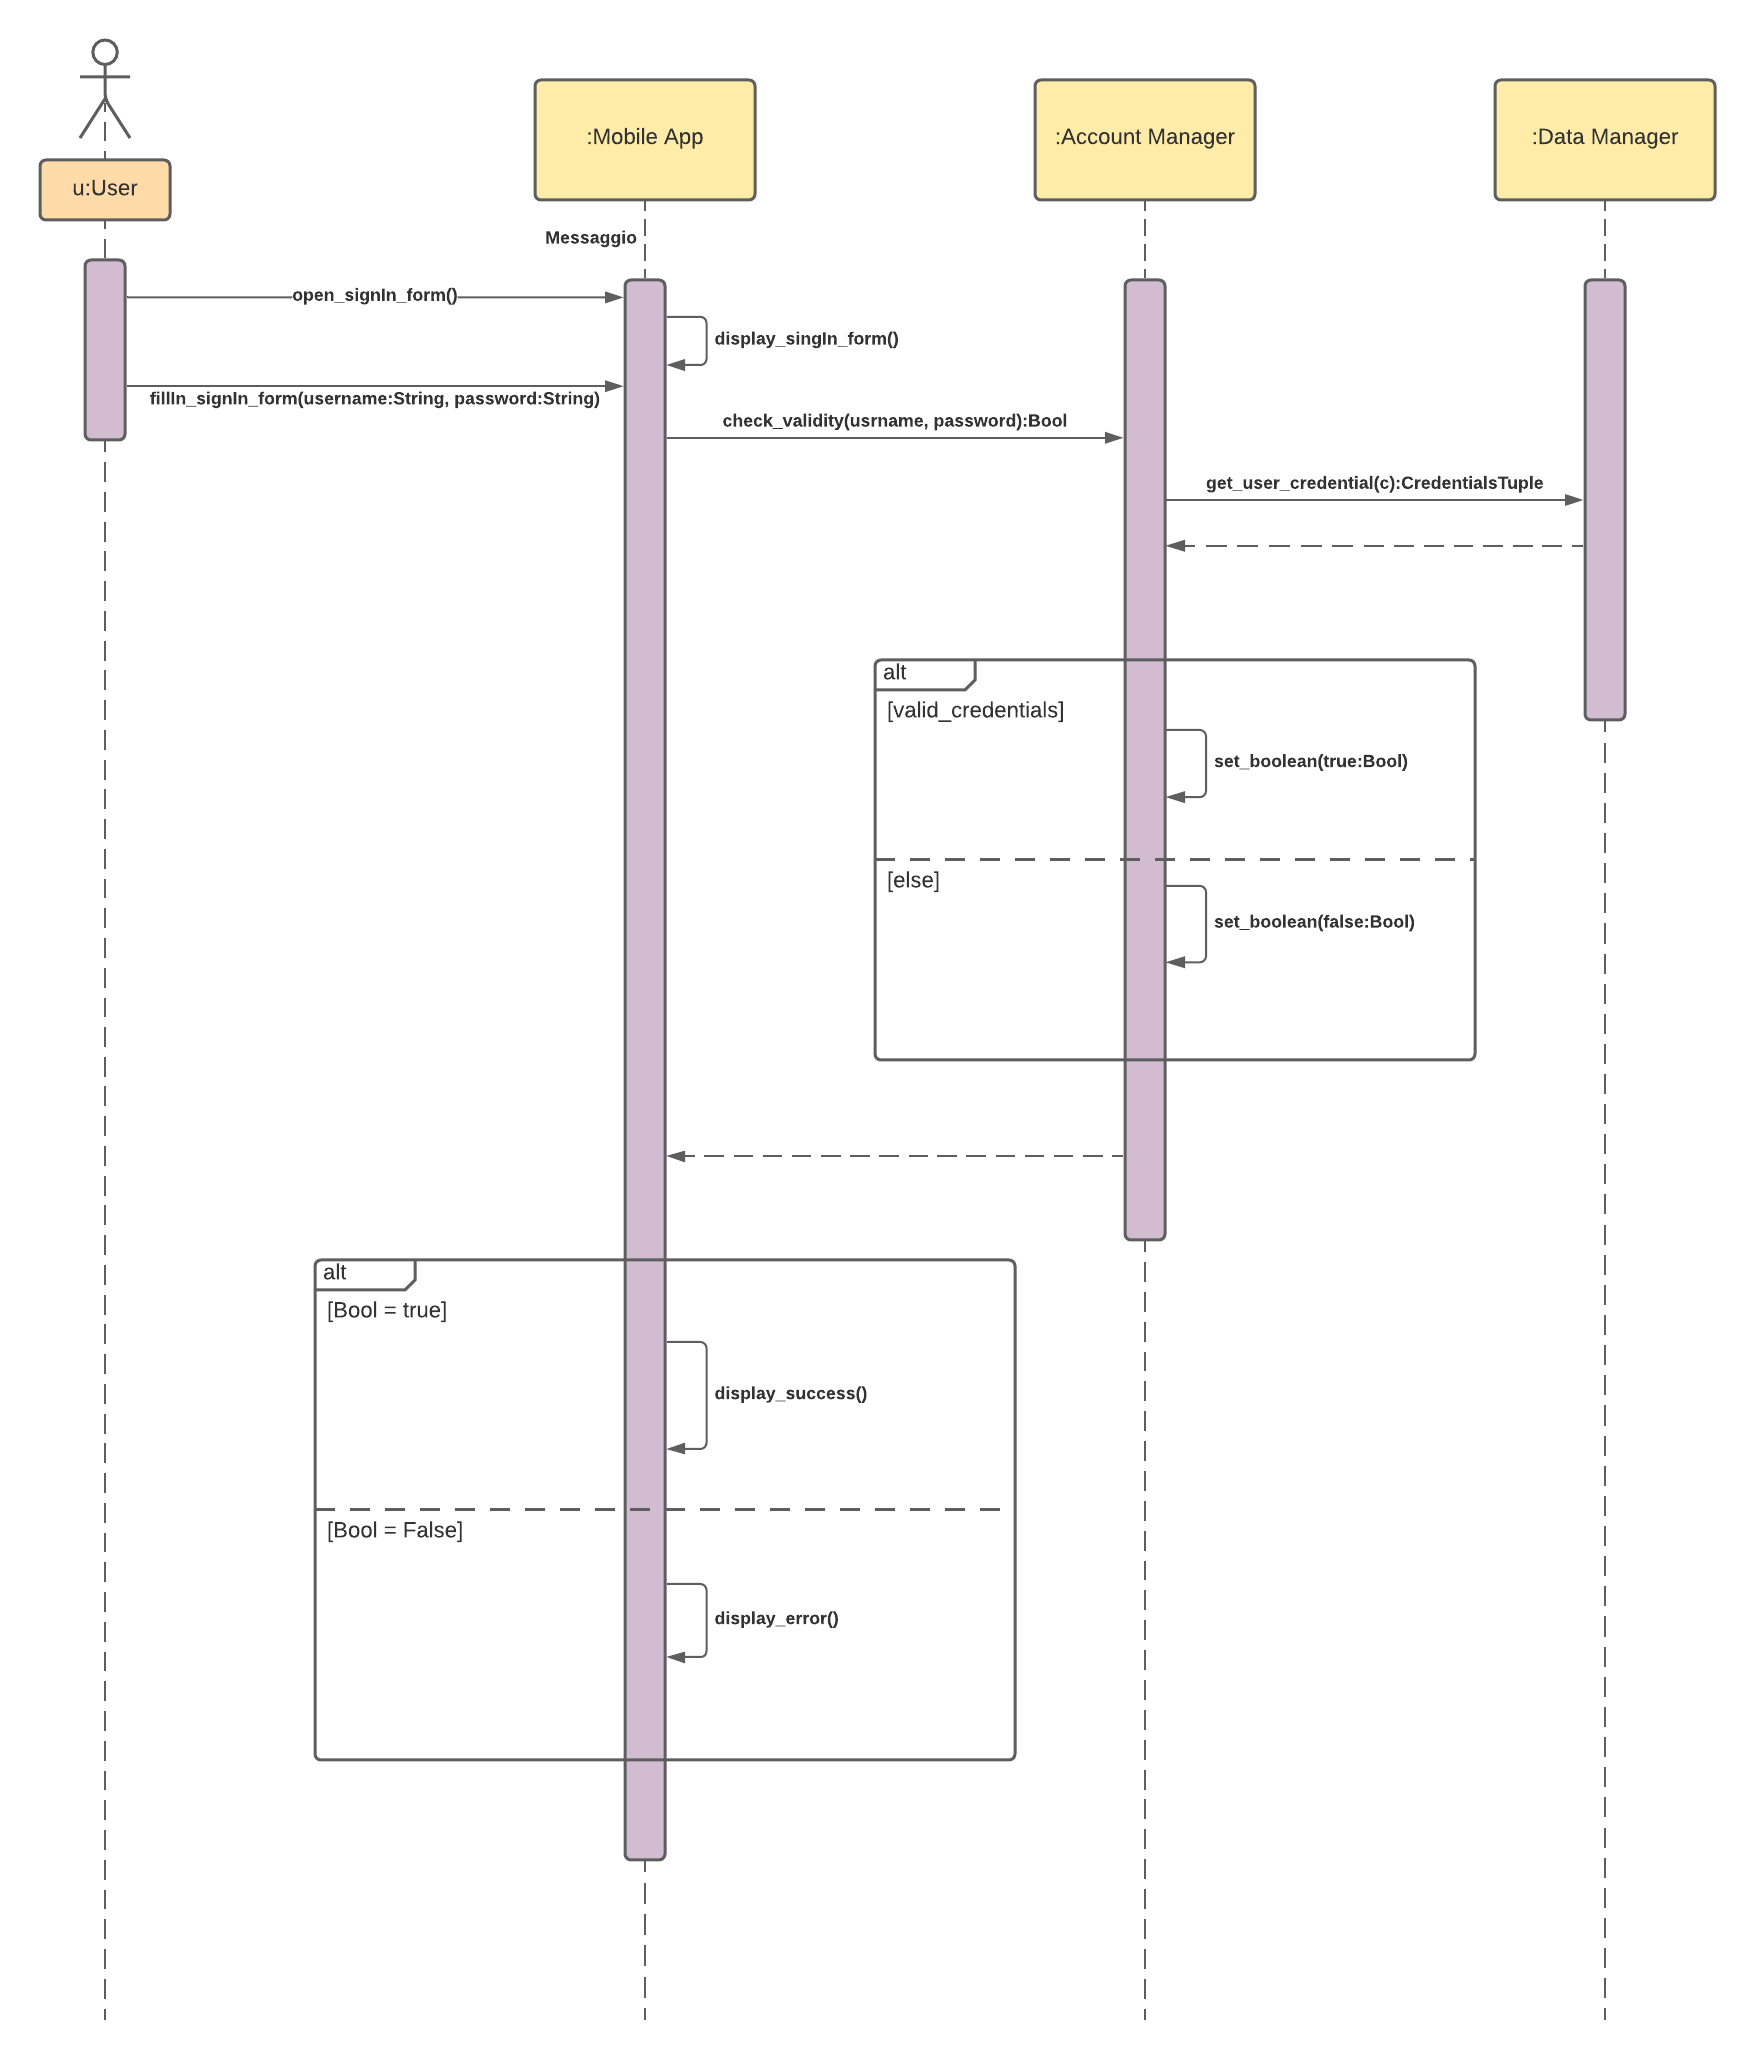
\includegraphics[width=1\textwidth]{Images/runtimeViewDD/RunTimeViewUserLogIn(1).png}
    \caption{\label{fig:RunTimeViewUserLogsIn}{1.User Logs In}}
\end{figure}

\begin{figure}[h!]
    \centering
    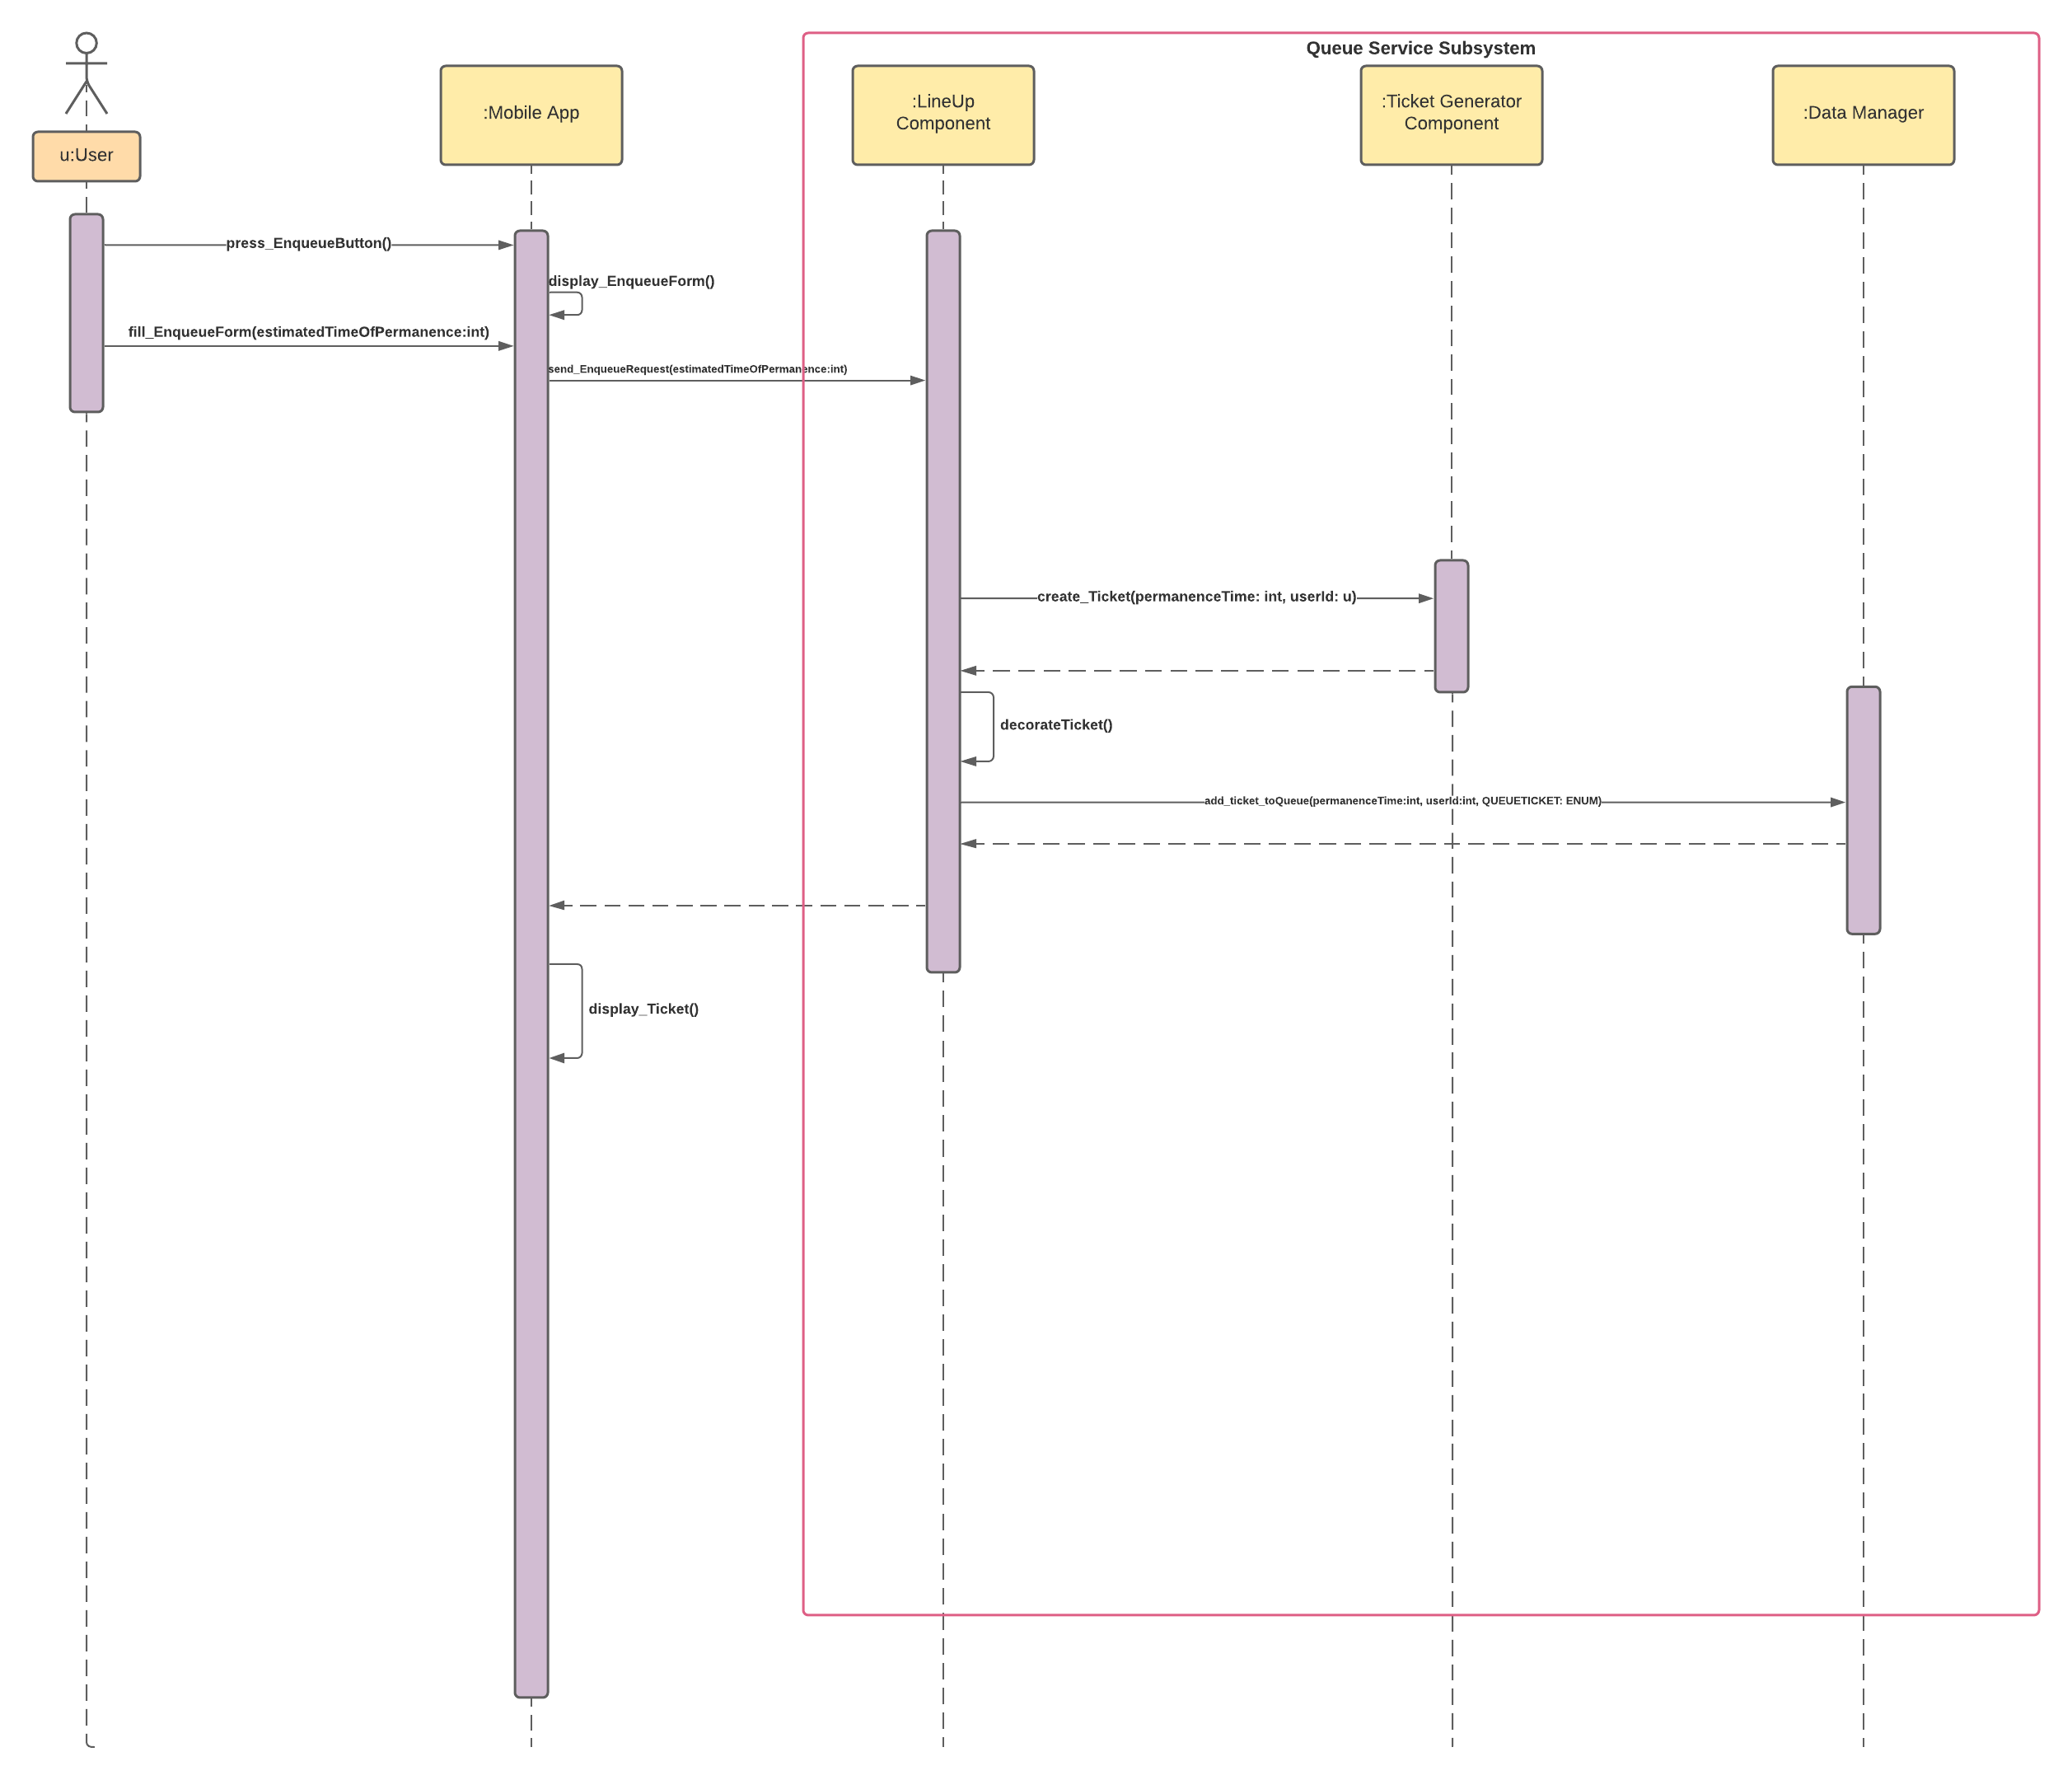
\includegraphics[width=1\textwidth]{Images/runtimeViewDD/RunTimeViewUserEnqueue.png}
    \caption{\label{fig:RunTimeViewUserEnqueue}{2.Customer Enqueues}}
\end{figure}

\begin{figure}[h!]
    \centering
    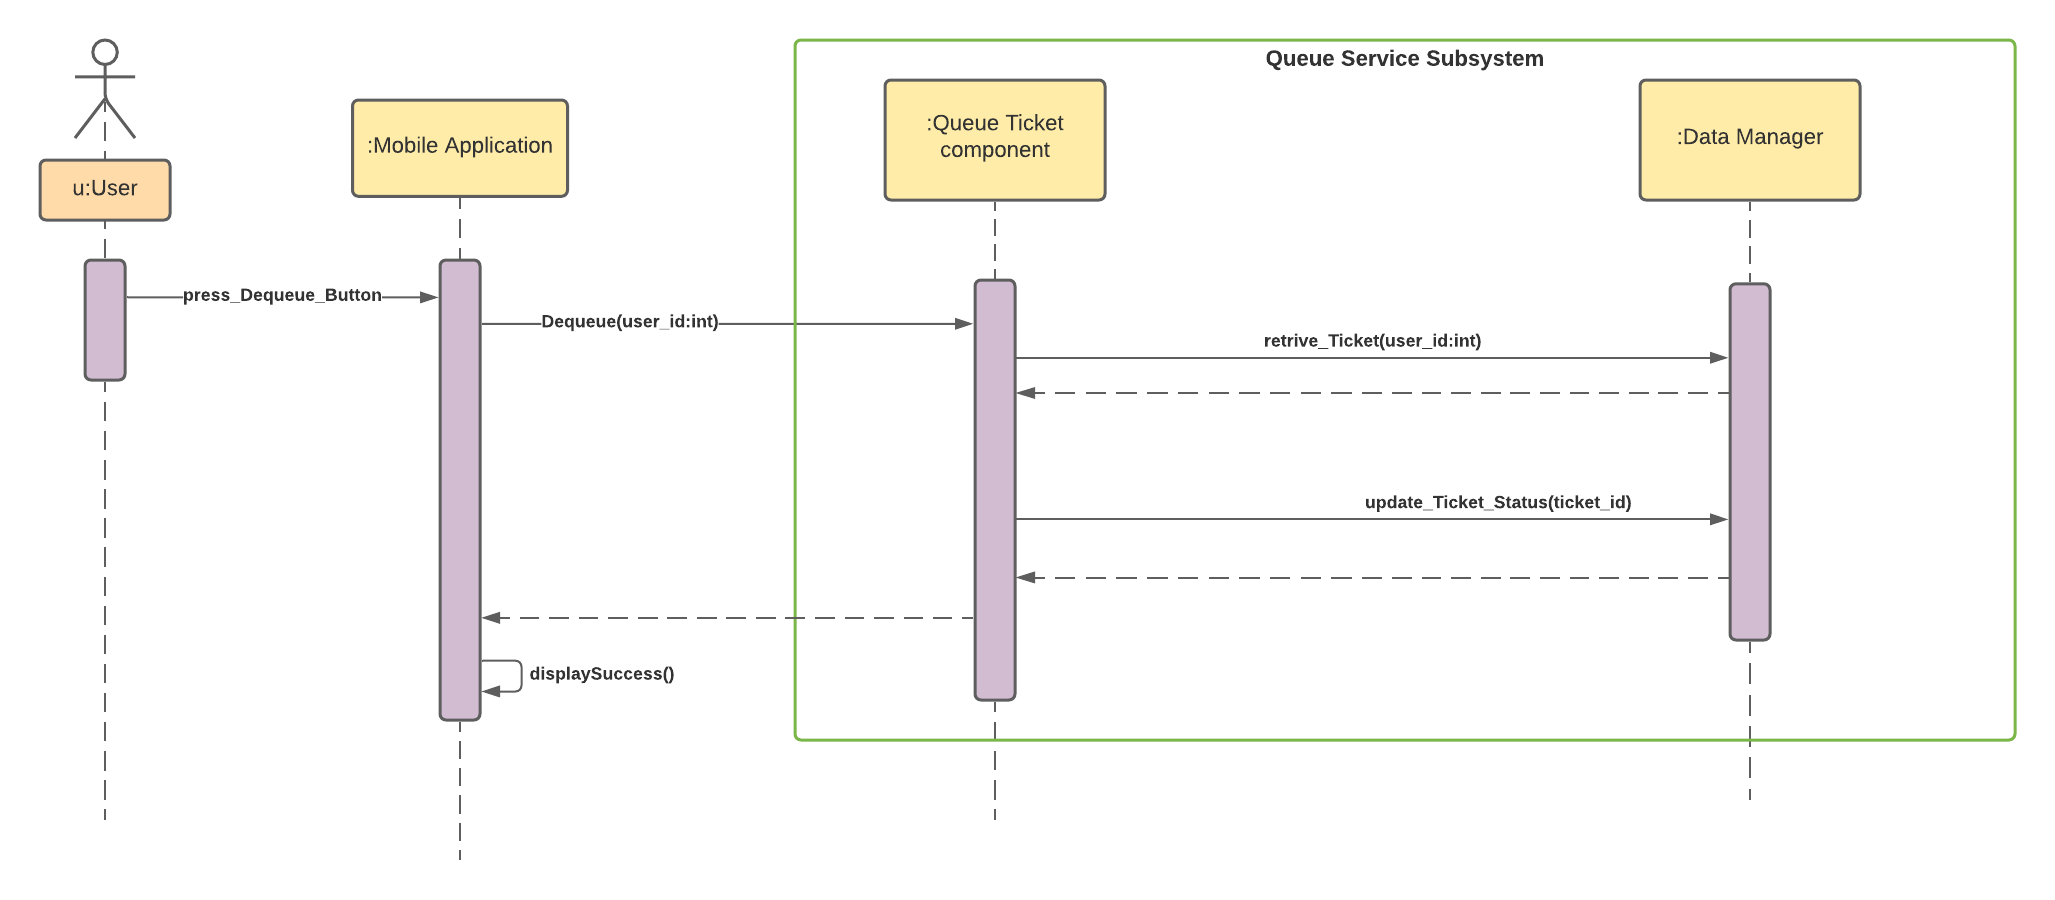
\includegraphics[width=1\textwidth]{Images/runtimeViewDD/RunTimeViewDequeue.png}
    \caption{\label{fig:RunTimeViewDequeue}{3.Customer Dequeues}}
\end{figure}

\begin{figure}[h!]
    \centering
    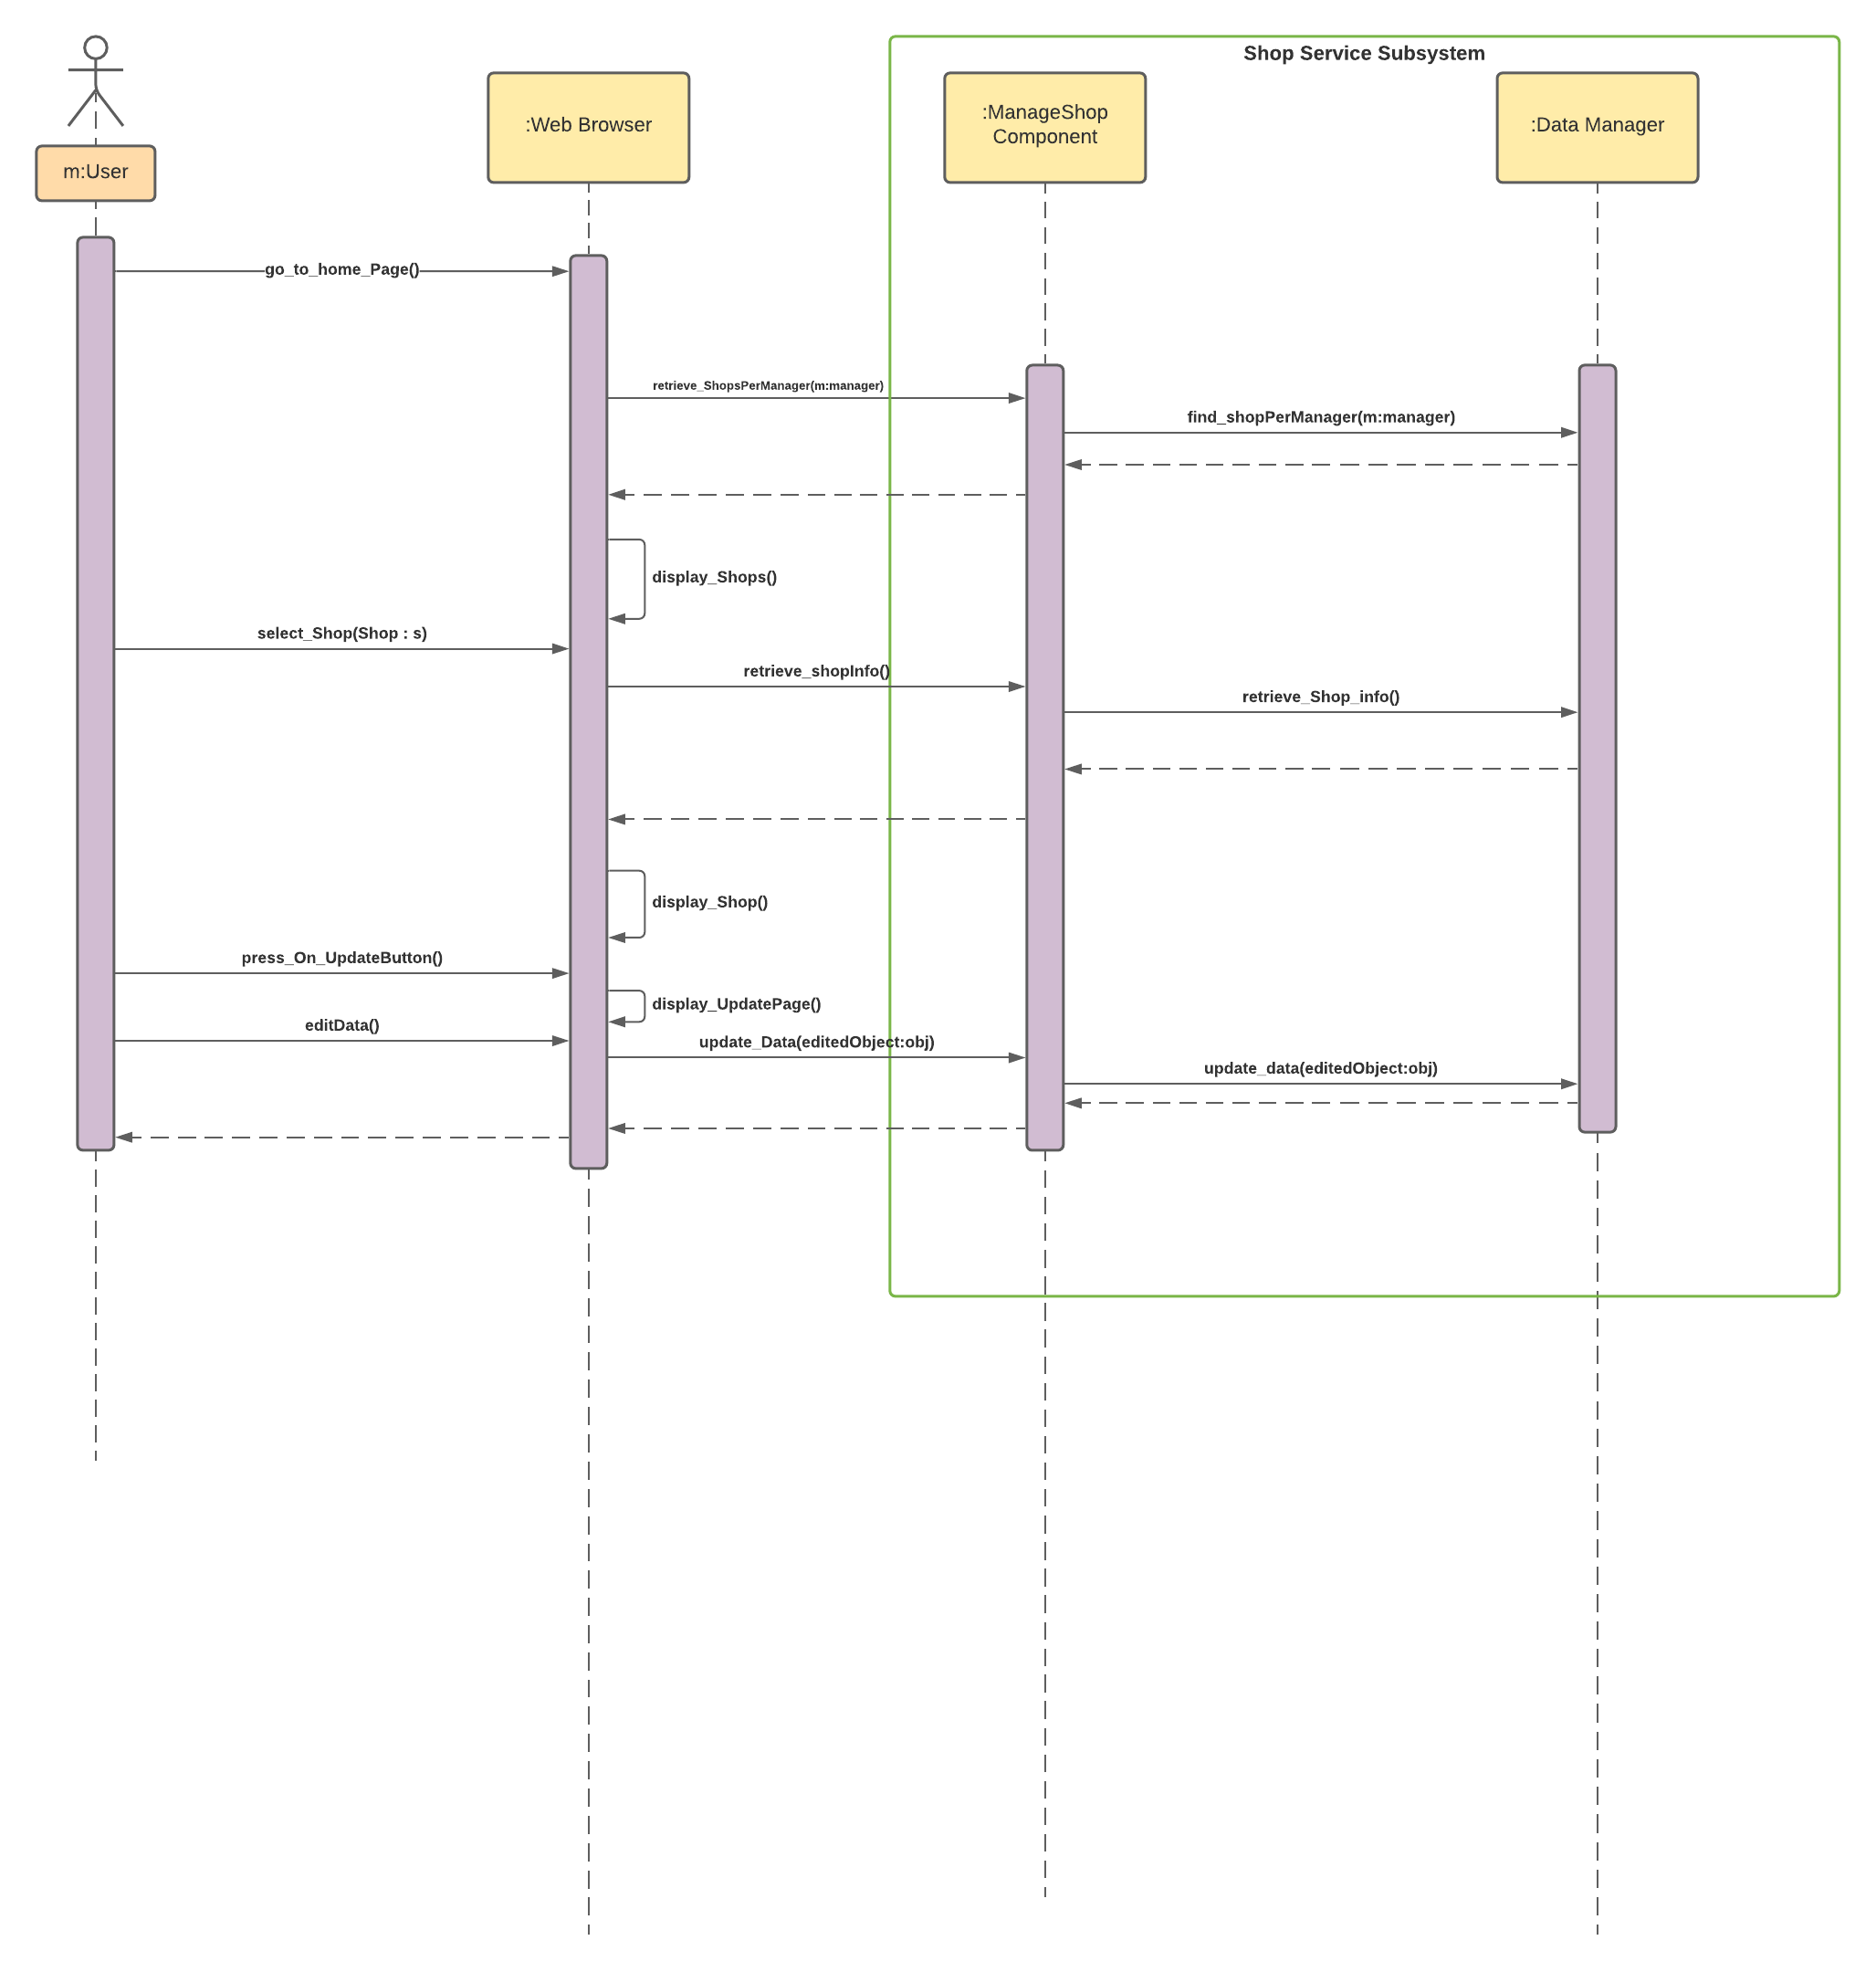
\includegraphics[width=1\textwidth]{Images/runtimeViewDD/updateshopruntime.png}
    \caption{\label{fig:RunTimeViewUpdateShopEnqueue}{4.Manager Updates Some Shop Information}}
\end{figure}

\begin{figure}[h!]
    \centering
    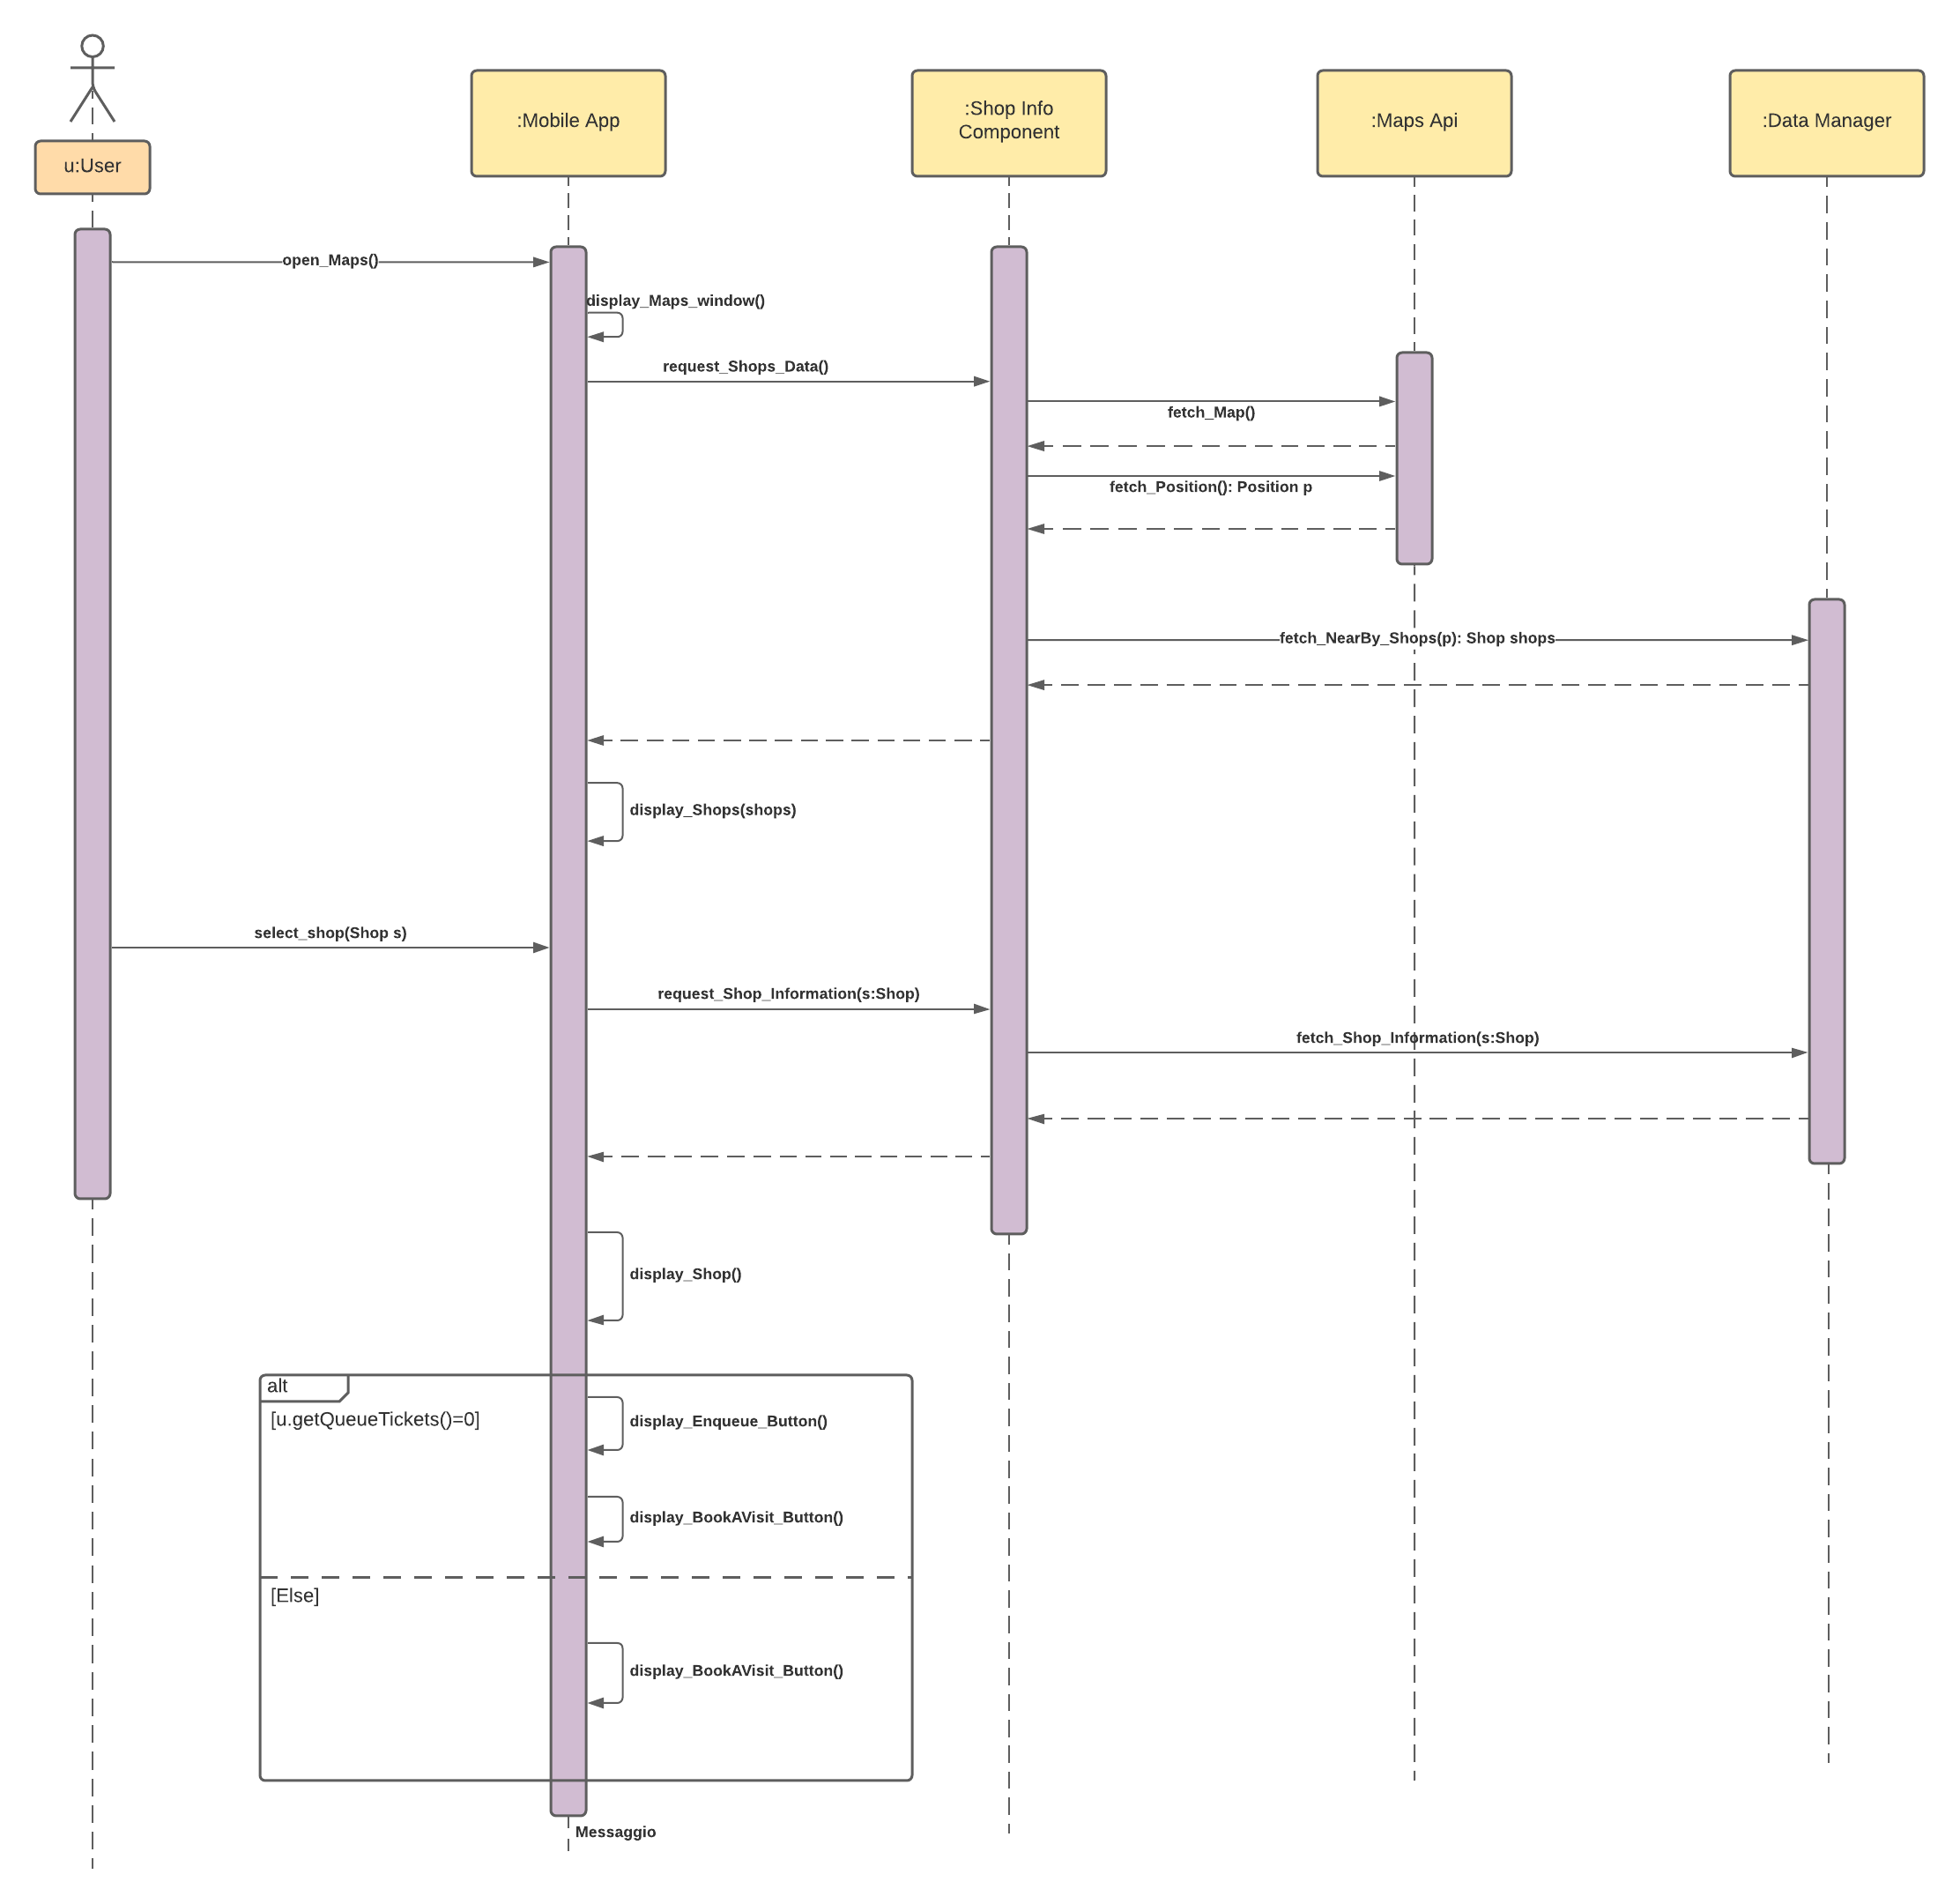
\includegraphics[width=1\textwidth]{Images/runtimeViewDD/RunTimeViewUserSearchAShop.png}
    \caption{\label{fig:RunTimeViewSearchesAShop}{5.User searches a Shop}}
\end{figure}

\FloatBarrier

\subsection{Component interfaces}
\label{subsect:componentinterfaces}

In this section we illustrate the main methods belonging to the interfaces of the components.

\begin{figure}[h!]
    \centering
    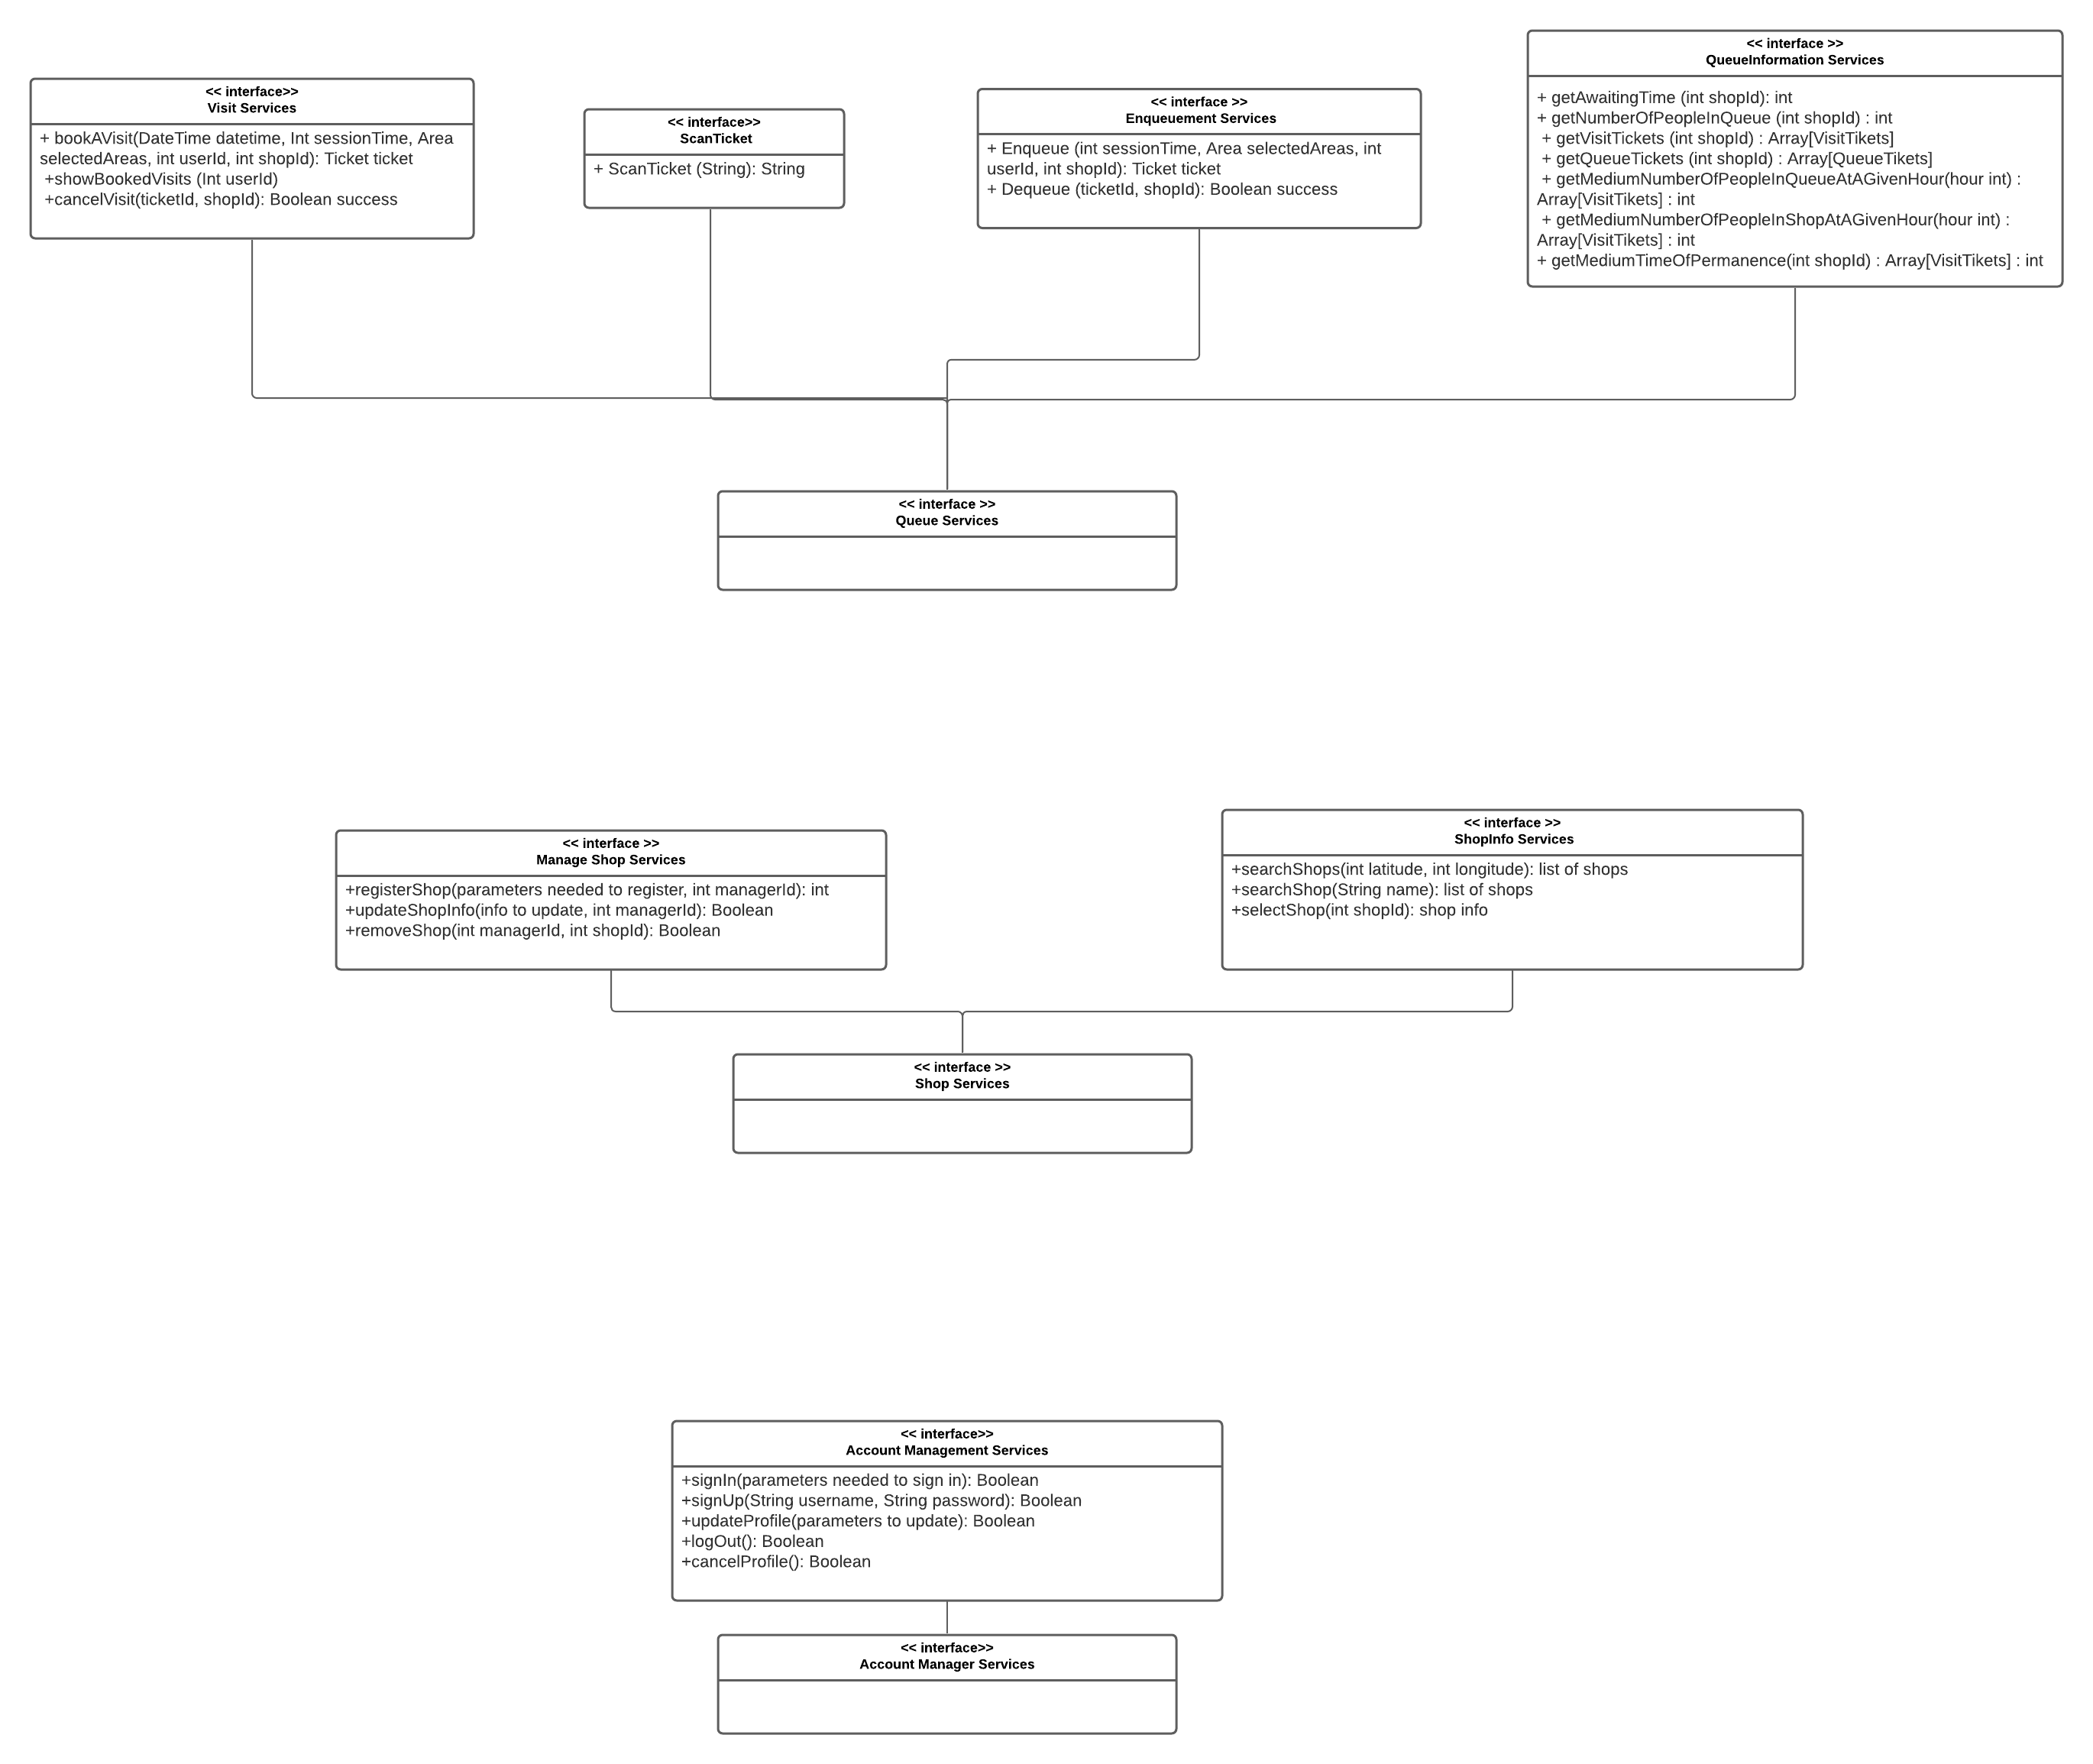
\includegraphics[width=1\textwidth]{Images/InterfacesDiagram.png}
    \caption{\label{fig:InterfacesDiagram}{Interfaces Diagram}}
\end{figure}

\FloatBarrier

The \textbf{Queue Service Interface} gathers all of the functionalities needed to interact with the queue of a shop and the tickets that compose it.\newline
Indeed, it offers the users the functions needed to manage enquements, visits, to retrieve information about the queue status, about their tickets and to inspect analytical data.
    
The \textbf{Shop Service Interface} gathers all of the features regarding the shops. Thus, it is the proxy through which a manager can register their shops on our system and to update them later on. It also offers methods that allow to retrieve all of the desired information about a shop, such as its position or the items that it sells.

The \textbf{Account Manager Interface} as clearly as its name may suggest- may I add, once again- this interface offers to the user all of the features related to their accounts. Examples of methods offered by this interface are "Sign In", "Log in" and "Update Profile".

\subsection{Selected architectural styles and patterns}
\label{subsect:selectedarchitecturalstylesandpatterns}

In the following, we have individuated a series of desing and structural pattern which may be selected in a future implementation of CLup.

\begin{itemize}[topsep=0pt]
    \item \textbf{Selected Design Patterns}
        \begin{itemize}[topsep=0pt]
            \item \textbf{State Pattern}: allows an object to behave different according to the circumnstances. It is used to implement the status of the tickets.
            \item \textbf{Facade Pattern}: an objects which, through an easier interface, allows the access to several subsystems offering more complex and variagate interfaces.
            \item \textbf{Adapter Pattern}: allows interoperability within different interfaces. This will be used for the interaction of the Qr-code application implemented by us with the underlaying system, since the latter isnt known \textit{a priori} and can differen accordingly with the preferences of the managers.
            \item \textbf{Factory Pattern} In class-based programming, the factory method pattern is a creational pattern that uses factory methods to deal with the problem of creating objects without having to specify the exact class of the object that will be created. This can be in the optic of extending the range of tickets to be offered to the clients in the future.
            \item \textbf{Decorate Pattern} In class-based programming, allows to add functionalities to an exisiting object at runtime.
            In a optic of growth of the application, it can be a wise choice to add new functionalities to the tickets, such as readapt them as coupons or as fidelty cards.
            \item \textbf{Chain of Responsability Pattern}  In this design pattern a request from a client can be handled by a number of handler or receiver objects. So basically, the client request is passed down each handler in the chain until a handler that can process the request is found. Servlet filters are a classic example of the Chain of Responsibility pattern. Spring has a class called HandlerInterceptorAdapter which is also an example of the Chain of Responsibility pattern. It has a method called preHandle, which follows the chain of responsibility pattern. Both servlet filters as well as Spring interceptors can be used to house code that is common for all requests like logging or authentication and that is separate from the business logic. We chose this to boost security aspects of CLup.
            \item \textbf{Observer Pattern} is a pattern according to which an object, named the subject, mantains a lists of its dependents, called observers and notifies them automatically at any state change. It will be used for implement the push notifications and along with the MVC pattern explained right after this.
        \end{itemize}
    \item \textbf{Selected Structural Patterns}
        \begin{itemize}[topsep=0pt]
            \item \textbf{Model View Controller}: is a very common pattern which separate the presentation logic of the application from the business logic. It is a very popular and effective way to decouple the different parts of the system.
        \end{itemize}
\end{itemize}



